\section{Antinuclei in the cosmos}
Antinuclei are some of the rarest stable objects in cosmic rays, in fact, no compound antinuclei have ever been conclusively observed in cosmic rays. But it is this exact fact that makes them such promising candidates for the search of new physics. Whereas for other particle species the signal to background ratio might be miniscule for any new effect, antinuclei production is so rare in standard model processes that any new physics might produce signals orders of magnitude greater than what can be explained with our current knowledge. And while no conclusive observation of antinuclei in cosmic rays has been published, the AMS-02 Collaboration has repeatedly reported signals of antihelium\cite{}, motivating a renewed push of research interest into cosmic ray antinuclei. \\
The goal of this section is to discuss two possible exotic sources of antinuclei in our galaxy: i) WIMP dark matter and ii) extragalactic WIMP dark matter. These are compared to antinuclei produced in high energy cosmic ray collisions with the interstellar medium, which is an analogous process to the one used to produce antinuclei at accelerators. Crucially, the new measurements of the inelastic cross sections of antihelium laid out in section \ref{sec:ResHe3SigmaInel}, and the first low energy measurements of the antideuteron-matter inelastic cross section laid out in \cite{antideuteronXS}, are for the first time incorporated in such studies. The discussion therefore focuses in particular on propagating these measurements to obtain the experimental uncertainites from inelastic interactions on the antinuclei flux near earth.\\
In order to study the two sources we employ the GALPROP framework. This framework propagates particles through our galaxy, simulating various effects such as diffusion, convection and also annihilation. The resulting fluxes near earth are then presented for both antideuterons and \ahe, for different dark matter masses and profiles, and the significant differences and similarities are discussed. Finally, current and planned experiments for detecting antinuclei in cosmic rays are discussed. 

\subsection{Sources of antinuclei in the cosmos}
Antinuclei are some of the rarest stable particles in our galaxy, since very few abundantly occurring processes will produce them in any non-negligible amount\cite{}. This is in contrast to nuclei, which are the most abundant stable particleswithin our galaxy. A large amount of the light matter nulcei (up to Lithium) was produced during Big Bang Nucleosynthesis (BBN)\cite{}, while all heavier nuclei were produced during stellar nucleosynthesis\cite{}. However, due to the asymmetry of matter and antimatter in our galaxy, neither of these methods is thought to be a dominant source for antinuclei. Antimatter produced during BBN is likely to have annihilated propagating through the galaxy from the Big Bang until today, and since we have no evidence that anti-stars exist\cite{}, it is unlikely that antinuclei could be produced through stellar nucleisynthesis. \\
We therefore have to look to other processes which could produce antinuclei. Due to baryon number conservation, all such processes are likely to produce at least an equal amount of light nuclei as well. However, since nuclei are far more abundant than antinuclei, these processes will only contribute a negligible amount to the total nuclei flux in our galaxy, while they might dominate the antinuclei flux. This extremely high expected signal to background ratio is the reason why antinuclei are considered such a promising probe into new physics.

\subsubsection{High energy cosmic ray collisions}
The most well known source for antinuclei in cosmic rays -- and the only one which does not require new physics or as of yet undiscovered objects -- are collisions of high energy cosmic rays with the interstellar medium. Such collisions, akin to collisions at particle accelerators, will produce antinuclei by converting the available mass-energy from the collision into (anti-)nucleons which then coalesce. Given the collisions systems which dominate such reactions (combinations of protons and Helium nuclei both in the projectile and the target), and the need to conserve the baryon number, it is necessary to produce at least 4 (6) new particles in order to produce antideuterons (\ahe). This fact -- combined with the highly boosted frame of these collisions which results in significantly less available phase space -- means that the cross sections of these events are small, and the conditions are difficult to reproduce at accelerators with sufficient statistics to fully constrain the production. So while the energy threshold for these reactions can be calculated exactly, the shape and normalization of the production spectrum is not completely constrained, leading to uncertainties of about an order of magnitude. This uncertainty is in part also due to the fact that collisions at particle accelerators don't perfectly reproduce the conditions in such high energy collisions with the interstellar medium in terms of rapidity. The observations observed at accelerators probe antinuclei production at mid-rapidity, while such collisions produce them mainly at forward rapidity, and the rapidity dependence of the antinuclei production cross section is not precicely know\cite{}.CHECK THIS \\

The production of antinuclei in these high energy cosmic ray collisions also suffers from the challenge that the range of energies of the projectiles is by definition huge, since effectively the entire spectrum of cosmic rays needs to be taken into account. Therefore, the differential production cross section at each projectile energy needs to be folded with the amount of cosmic rays at this energy. This is usually done by employing event generators, which take the centre of mass energy as input and produce nucleons in the centre of mass frame. The coalescence model (as discussed in section \ref{sec:IntroProductionAntinuclei}) is then used in order to obtain the antinuclei spectrum from these produced nucleons. In order for this to occur, the nucleons produced by the event generator need to be close enough in phase space in order to meet the coalescence condition. If only very few nucleons are produced, this is obviously a very rare situation, and thus the production cross-section decreases. Another way to say this is that the coalescence parameter scales as a function of multiplicity \cite{}. As a result of the rarity of this process at lower energies (PLACEHOLDER, GET A NUMBER), drastic amounts of Monte Carlo simulations are needed in order to obtain an estimate for the production cross section at even a single point of the spectrum, and even more so for the entire spectrum. This is only exacerbated for each additional nucleon added. This yields the second uncertainty for the production in high energy cosmic rays, which is the statistical uncertainty on the estimates for the production cross section.\\

\subsubsection{Weakly interacting massive particles (WIMPs) - dark matter}\label{sec:WIMPS}
Some WIMP dark matter theories predict that WIMP annihilations can produce a significant amount of antinuclei \cite{}. This can be understood simply from the available energy in such a process. A cold dark matter particle pair annihilating has \Vs\ = $2\mathrm{m}_\chi$. The net baryon number would be 0 in such a process, resulting in no further penalty for the production of multiple antinucleons. Per definition, WIMPs interact only weakly, and thus their initial annihilation would occur through a weak channel. Since the weak bosons couple to all other standard model particles, this enables the production of other  standard model particles, such as antinuclei. \\

The spectrum and yield of antinuclei produced in these annihilations has to be estimated based on known standard model processes. To this end, Monte Carlo event generators are employed\cite{}, in which the initial state is the first state of standard model particles (such as W$^+$W$^-$ or b$\overline{\mathrm{b}}$) which is assumed to occur in the annihilation process, with a COM energy equal to twice the dark matter mass \dmm\. Since event generators do not produce (anti)nuclei -- but only the individual nucleons -- the (anti)nuclei yields and spectra have to be calculated using the coalescence model\footnote{See Appendix \ref{App:statHadronModel} for an explaination of why the statistical hadronization model cannot be used to calculate (anti)nuclei yields from dark matter annihilations}.  \\ 

The WIMP dark matter is assumed have been in thermal equilibrium with luminous matter after the Big Bang, and is believed to be responsible for the anisotropies seen in the cosmic microwave background (CMB) \cite{}. Since then, however, the dark matter would have cooled with the expanding universe, and thus is assumed to be at a similar temperature as the CMB today. This is referred to cold dark matter. Another consideration which supports cold dark matter is that the majority seems to be gravitationally bound within galaxies. As such, the COM frame is assumed to be the same as the galactic frame, and no boost from the initial velocities are necessary. This is convenient, since one can therefore simply take the spectrum of produced antinuclei per dark matter annihilation -- which is obtained from applying a coalescence afterburner to the output of a Monte Carlo event generator -- and multiply it by the local annihilation rate of dark matter. Thus, one can write the source term $q(\vec{r}, E)$ for WIMP dark matter as is written in equation \ref{eq:DM_source_term}. 

\begin{equation}\label{eq:DM_source_term}
    q(\vec{r}, E) = \frac{1}{2} \left( \frac{\rho_{\chi}(\vec{r})}{m_\chi}\right)^2 <\sigma v > \frac{dN}{dE}
\end{equation}

where the factor $1/2$ comes from symmetry considerations for majorana dark matter\footnote{See section \ref{sec:IntroMajoranaDiracDM} for a discussion on the difference between Majorana and Dirac dark matter.}, the term $\left( \frac{\rho_{\chi}(\vec{r})}{m_\chi}\right)^2$ is the square of the number density of the WIMP dark matter, which is then multiplied by the velocity averaged dark matter annihilation cross section $<\sigma v>$, giving the rate of dark matter annihilations for a given point in space. The final term of equation \ref{eq:DM_source_term} is the spectrum of produced antinuclei normalised to a single dark matter annihilation. The terms of equation \ref{eq:DM_source_term}, their contraints and degeneracies are discussed below.\\

The dark matter density profile $\rho_\chi(\vec{r})$ affects both the total amount of antinuclei produced as well as their initial distribution. This parameter can be constrained from measurements of the milky way's rotation curve, similarly to how it is done for other galaxies. However, measuring the rotation curve of the Milky Way involves extra challenges, given that we are measuring from within. For other galaxies, the rotational velocities of the stars can be measured from their red/blue shift, and their position in respect to the galactic center is easily estimated by their angular displacement. For stars in our own galaxy, we cannot purely rely on the angular position of a star in the sky in order find the displacement of the star in respect to the galactic center, as the star could be anywhere in the galactic plane within this line of sight. This is illustrated on the right of figure \ref{fig:measuringDarkMatterProfiles}. It is therefore necessary to determine not only position in the sky, but also the distance to the star in question. Similarly, the rotational velocity of the stars has to take into account that through the red/blueshift of the spectral lines we can only measure the velocity component parallel to our displacement. In order to reconstruct the required full 3-d position and velocity we further require the distance to the object and its "proper motion", which is the angular speed at which it moves along the sky normal to its displacement to earth. This proper motion is usually measured in arcseconds/year. The consequence of these difficulties is that the uncertainty on both the position and rotational velocity of stars increases the further away from earth the star is positioned, and becomes further more difficult for stars at greater distances to the galactic centre than the sun. Our galaxy's rotation curve  has been reported in \cite{}, found by combining multiple existing measurements. It is reproduced in figure \ref{fig:MilkyWayRotationCurve}. \\

\begin{figure}[h]
    \centering
    \includegraphics[width=0.45\textwidth]{}
    \includegraphics[width=0.45\textwidth]{}
    \caption{Left: This shows the method for measuring the rotation curves for galaxies other than the milky way. The displacement from the center of the galaxy is measured by measuring angular displacement. The rotational velocity can be extracted by measuring the red/blue shift of the star\cite{}. Right: This diagram shows the method for measuring the rotational velocity and position of stars within our galaxy.}
    \label{fig:measuringDarkMatterProfiles}
\end{figure}

\begin{figure}[h]
    \centering
    \includegraphics[width=0.45*\textwidth]{}
    \caption{Rotation curve of stars in the Milky Way, as a function of distance from the galactic center.}
    \label{fig:MilkyWayRotationCurve}
\end{figure}

In order to fit such rotation curves, our galaxy is conventionally split into individual parts, each of which can be assumed to have a simpler shape. The usual breakdown of these parts is shown in table \ref{tab:MilkyWayBreakdown}, and further details can be found in \cite{Sofue_2016}. The gravitational potentials of these parts can then be summed up linearly, and the rotational velocities caused by each such potential can be added in quadrature. In order to fit the contribution from dark matter, the shape of the dark matter distribution has to be chosen a priori, such that the exact parameters and normalization can then be obtained from the fit. This is an important point, since the total normalization of the dark matter profile is not well constrained. Rather, the relatively well constrained rotation curve in the proximity of the solar system results in the fact that the local dark matter density $\rho_\chi(\vec{r}=r_\odot) := \rho_\chi^\odot$ is much better constrained than the total normalization of the dark matter profile. Thus, the different dark matter profiles are constrained to their value at $r_\odot = 8.5$kpc\footnote{The value is currently estimated to be 0.5GeVcm$^-3$ \cite{}.}, the estimated position of our sun. \\
\begin{table}[h]
    \centering
    \begin{tabular}{|c|c|c|c|}
        \hline
        Part & Shape & Extent & Total Mass \\
        \hline
        Central black hole & Point mass & $<$ 0.1pc & 3.6\times 10$^6$ M$\odot$ \\
        \hline
        Buldge(s) & Spherical exponential & $<$1kpc & 10$^11$ M$\odot$ \\
        \hline
        Flat disk & Constant flat disk & $<15$kpc & xx M$\odot$ \\
        \hline
        Dark matter halo & vaires & 100s of kpc & 10$^12$ M$\odot$ \\
        \hline
    \end{tabular}
    \label{tab:MilkyWayBreakdown}
    \caption{Individual axissymmetric parts of the Mikly Way used for fitting rotation curves. The distinction is made in order to simplify the fit, rather than a hard distinction within the actual galaxy. Non-axissymmetric components are neglected for rotation curves, based on the assumption that any effects would cancel out when averaged over the full rotation. The values for the total mass were taken from \cite{Sofue_2016}. The extent column is approximate and given in order to help the reader visualise the distributions. Due to the distributions being exponential, they don't really go to 0.}

\end{table}

There are several profiles on the market, which achieve similar goodness-of-fit when fit to account for the dark matter component in the rotation curve\cite{}, while also achieving the required normalisation at $r_\odot$. The ones used in this work are the Navarro-Frenk-White(NFW) profile\cite{}, shown in equation \ref{eq:NFW}, 

\begin{equation}\label{eq:NFW}
    \rho_\chi^{NFW}(\vec{r}) = \frac{\rho_0}{(r/r_s)[1+(r/r_s)]^2}
\end{equation}
with scale radius $r_s=$24.42kpc. The Einasto profile\cite{}, shown in equation \ref{eq:Einasto}, 

\begin{equation}\label{eq:Einasto}
    \rho_\chi^{Einasto}(\vec{r}) = \rho_0 \mahtrm{exp} \left\{ -\frac{2}{\alpha}\left[ \left( \frac{r}{r_s}^\alpha -1\right) \right] \right\}
\end{equation}
with $\alpha$=0.17 and $r_s$=28.44kpc, and the much shallower isothermal profile \cite{} and the isothermal profile, shown in equation \ref{eq:isothermal}
\begin{equation}\label{eq:isothermal}
    \rho_\chi^{isothermal}(\vec{r}) = \frac{\rho_0}{r^2+r_s^2}
\end{equation}
with $r_s$=4.38kpc. The profiles are plotted in figure \ref{fig:DMProfiles}, using best fit values taken from \cite{Ibarra}. It can be seen that the isothermal profile has a very shallow rise towards the galactic center, while the Einasto profile rises very steeply. The NFW profile lies between the two, and is often used preferentially \cite{}. These three profiles cover most of the available parameter space for the dark matter profile. \\

\begin{figure}[h]
    \centering
    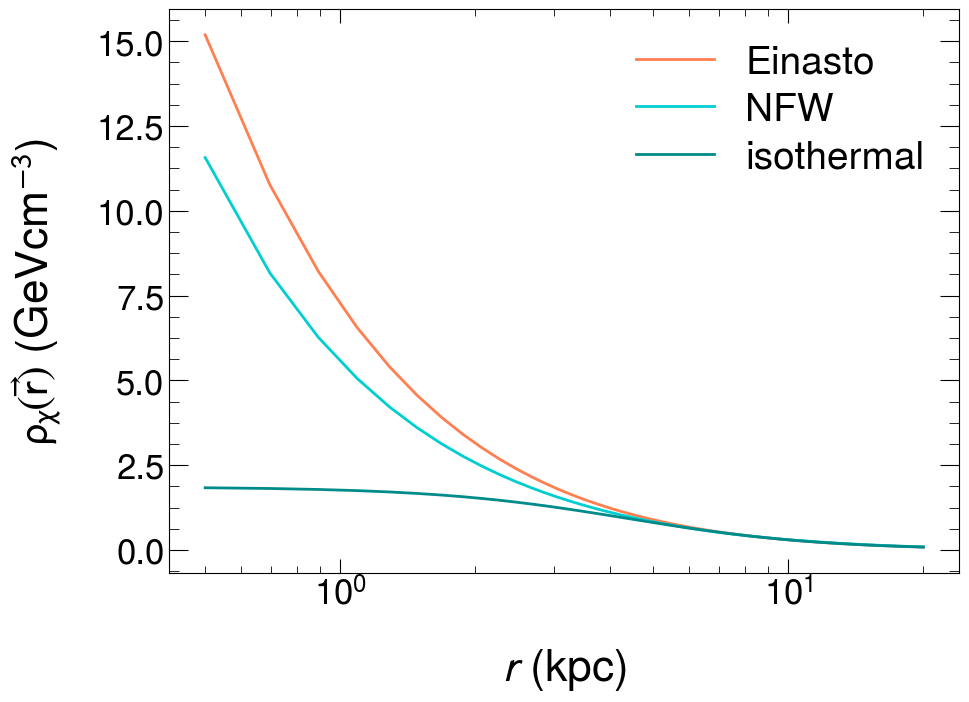
\includegraphics[width=0.8\textwidth]{figures/DMProfiles_distributions_log.png}
    \caption{Dark matter density profiles used in this work, as a function of the distance to the galactic centre. The best fit values for each profile are taken from \ref{Ibarra, IbarraSources}}
    \label{fig:DMProfiles}
\end{figure}

It is important to ask why the stark differences towards the center of the galaxy play such a reduced role that all three of these profiles are able to fit the data, and if such differences would therefore make any interpretation of an antinuclei flux from dark matter impossible. The answer to the first part of the question is twofold. Firstly, it is very challenging to measure the rotation curve of our own galaxy with high precision at positions far from the solar system. Secondly, the gravitational effect of the dark matter halo contributes mainly at larger distances from the galactic center, where the presence of extra mass at the centre of our galaxy (from a steeper profile) is not as strongly felt. The second question also has a fortunate answer: the effect of different profiles on a potential local flux of antinuclei from a dark matter source is rather small, as is discussed in section \ref{sec:ResDMProfiles}. \\

To summarize: the dark matter density profile in our galaxy is constrained by measurements of the milky way's rotation curve. Measuring the rotation curve is a non-trivial process, which involves measuring the 3d position of stars within our own galaxy. The most modern method to achieve this is Very-Long-Baseline-Interferometry (VLBI), which uses telescope arrays spanning continents as a giant interferometer. Once the rotation curve is measured, the effect from luminous matter is accounted for, and the remainder is assigned to the dark matter component. Due to the experimental uncertainties involved in measuring the velocity of far away objects, this leaves a significant plausible parameter space for the shape of the dark matter profile towards the center of our galaxy. 

The second term of equation \ref{eq:DM_source_term} is the dark matter mass, \dmm\ . The dark matter mass is a free parameter, with possible dark matter masses ranging from very light dark matter\footnote{A popular light dark matter model is the axion dark matter model \cite{}.} in the eV range all the way to the WIMP dark matter discussed in this work, with plausible mass ranges from 10s of GeV to the TeV range. As discussed in section \ref{sec:IntroWIMPs}, the appeal of WIMP dark matter is that the expected weak cross section of such a particle in the very early universe would yield a population today of the same magnitude as we observe. It would also explain the lack of evidence for the production of dark matter at accelerators, since we might at this point not yet have reached the energies required to produce such particles\footnote{Additionally, some supersymmetric partners could have exactly these required properties, which would make them suitable dark matter candidates\cite{}. However, the lack of evidence for supersymmetry makes this argument somewhat weaker than it was during the inception of WIMPs \cite{}}. Since the exact nature of dark matter remains a mystery, any mass within this WIMP range which is not excluded by other measurements can be assumed. The chosen mass has a direct effect on all three remaining terms of equation \ref{eq:DM_source_term}: i) $\frac{1}{m_\chi^2}$, ii) $\frac{dN_{\mathrm{\bar{p}, \bar{d}, {^3\overline{He}}}}}{dE}$  and iii)$<\sigma v>$. The effect on i) is trivial, and reduces the overall normalization of the antinuclei source term for higher \dmm\ . The mass' effect on ii) is based on the amount of energy available for the production of (anti)nuclei, as well as for their kinetic energy. For higher masses, the antinuclei yields increase non-trivially, but slower then the inverse square reduction from the first term. Additionally, the extra energy available for higher masses translates into a spectrum peaked at higher momenta. The effect on iii) is mostly experimental, since $<\sigma v>$ is constrained from antiproton measurements. Any dark matter annihilation process which can result in antideuterons must of course also produce antiprotons. However, contrary to heavier antinuclei, antiprotons are also copiously produced in other processes, due to the much lower energy threshold required for producing a single antinucleon, and the loss of the need to coalesce multiple antinucleons into a single compound antinucleus. This results in a significant and well constrained antiproton flux, which has been measured by the AMS collaboration \cite{}. Thus, any model choosen must not produce a dark matter component for antiprotons which is incompatible with those measurements. These limits are expressed in terms of $<\sigma v>$ as a function of \dmm\ . This representation is chosen since $\rho_\chi$ can be measured independently, and iii) varies much more slowly with \dmm\ than the other terms. The limits -- which have been extracted by several groups \cite{} and compiled by \cite{}-- are shown in figure \ref{fig:DMSigmaVLimits}. Indicated in the figure is the maximum limit on $<\sigma v>$, as extracted by several groups, as well as the "thermal value", which is the value expected in the early universe for a WIMP particle which would result in the currently observed abundance of dark matter. Also indicated in this figure is the region in which a possible excess of antiprotons was observed in the \pbar\ spectrum measured by the AMS collaboration, which could hint at a dark matter particle within this mass range of 50-100GeV/$c^2$. It can be seen from the left hand side of the figure that for low dark matter masses, the limits lie significantly below the thermal value for this cross section. Thus, \dmm\ affects the constraints on  $<\sigma v>$, particularly for low masses. It is also worth noting that these limits have to be extracted for a given dark matter density profile, and thus when exploring the maximum allowed antinuclei flux given the antiproton constraints, the choice of $\rho_\chi(\vec{r})$ is degenerate with the limits on $<\sigma v>$ set by the AMS antiproton limits.\\

\begin{figure}[h]
    \centering
    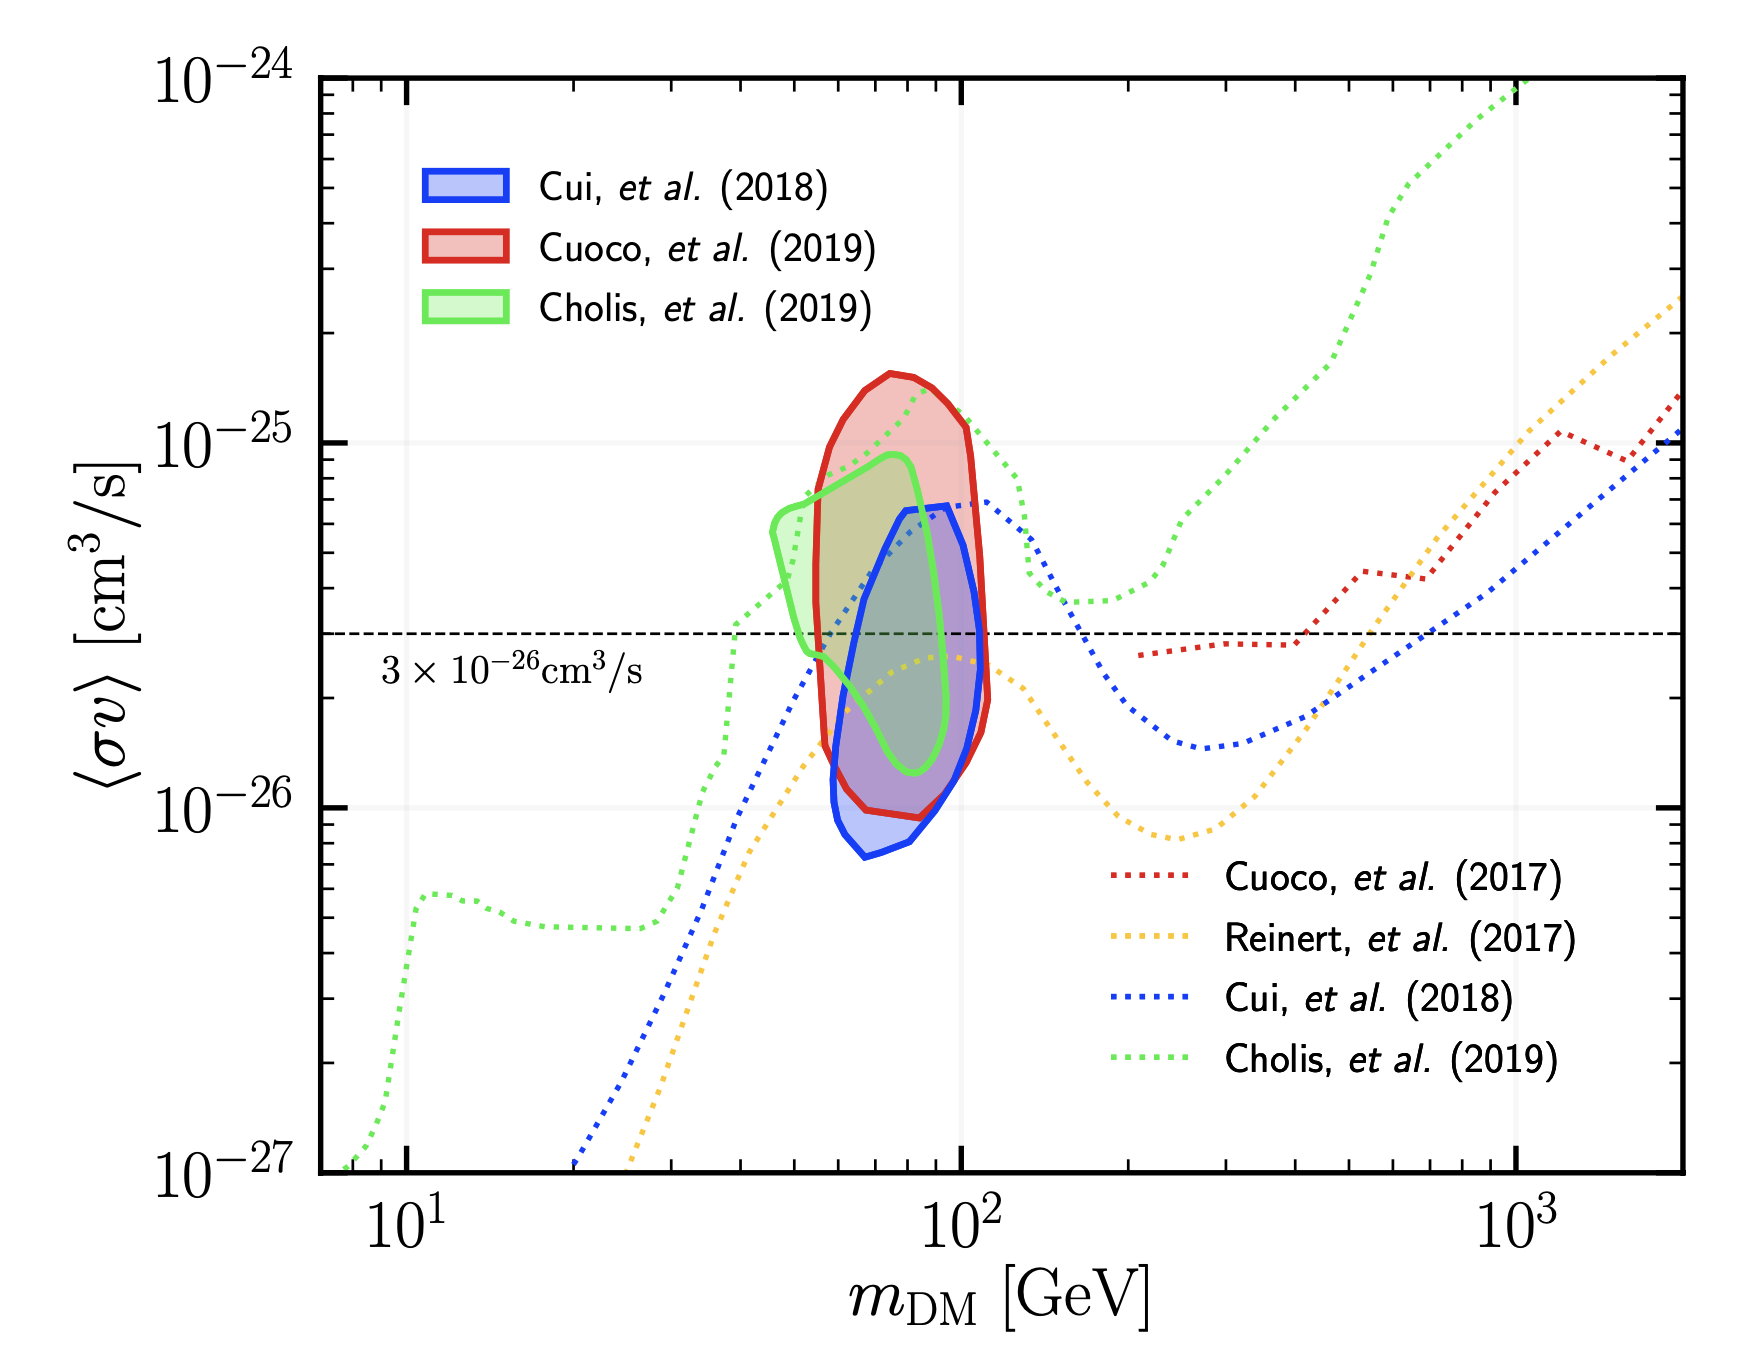
\includegraphics[width=0.8\textwidth]{figures/PbarLimitsAMS.png}
    \caption{Limits on  $<\sigma v>$ based on AMS antiproton data. Figure by \cite{} and reproduced here for easy of access.}
    \label{fig:DMSigmaVLimits}
\end{figure}

To summarise: WIMP dark matter models predict that dark matter can annihilate into antinuclei. The resulting antinuclei source term depends on 4 things: i) the dark matter density profile, ii) the dark matter mass, iii) the dark matter self-annihilation cross-section and iv) the produced spectrum of antinuclei, normalised to a single dark matter decay. i) is constrained by looking at the rotation curve of our galaxy, ii) is a free parameter, iii) is constrained from above by antiproton measurements as a function of \dmm\ and iv) is calculated based on coalescence models, which depend on the total available energy and thus \dmm\ . Thus, there are a few notable degeneracies between the different terms of this source function. However, current constraints on these parameters are not stringent and leave open a large, reasonable parameter space which could result in a measureable antinuclei flux from a dark matter source, affirming antinuclei studies as a great tool for the indirect search for dark matter.



\subsubsection{Extragalactic dark matter}
Dark matter is not exclusively bound within galaxies, but is also present in larger cosmological structures, such as galaxy groups. However, the profiles commonly used in order to fit the distribution of dark matter within our galaxy only take into account galactic dark matter, which can be inferred from the fact that such profiles go to 0 at large distances from the galactic centre. This is because to first order, the extragalactic component will vary over length scales bigger than our galaxy, so the gravitational potential caused by the extragalactic dark matter will be roughly constant within our galaxy, thus causing no active force which could be measured. However, such an additional flux of dark matter could indeed annihilate within our galaxy, thus providing an additional source for antinuclei. In this section the difference of this source to the galactic WIMP dark matter source will be qualitatively discussed. \\ 

In order to determine weather the antinuclei flux caused by extragalactic dark matter follows the same assumptions as the galactic component, it is necessary to examine the differences between galactic and extragalactic dark matter. The first difference would be their velocity. Since the galactic component is bound and the extragalactic is not, the extragalactic component's velocity must exceed the escape velocity of the Milky way, which lies at about 600km/s. This change in velocity may affect 2 terms in equation \ref{eq:DM_source_term}: the self annihilation cross section and the spectrum of produced antinuclei due to the boosted frame in which the collision takes place. \\
Starting with the effect on the self annihilation cross section, the difference might be due to the momentum dependence of the s-wave and p-wave contributions. The s-wave is velocity independent, while the p-wave contribution has a square dependence on the velocity. However, the speeds of 600km/s still only equate to a beta of 0.002, thus the contribution of the s-wave still dominates at these speeds, resulting in no change in regards to galactic dark matter. In a similar fashion it can be shown that the effect of the increased speed on the produced antinuclei spectrum is negligible. \\

The effect which remains is that of the overall normalisation, which is influenced by the extragalactic component to $\rho_\chi$. This extra component would have little to no effect on the rotation curve of our galaxy, and therefore causes a positive offset in comparison to the purely galactic case. The exact nature of this offset should to first order be roughly constant over our galaxy, however, the interaction of the extragalactic dark matter with our galaxy's gravitational pull would cause an increase in the local extragalactic dark matter density in comparison to another point within the local group. Thus, the main difference between the extragalactic dark matter and the galactic dark matter is the consideration of where the majority of annihilations would occur. Finally, we can conclude that since the overall normalisation for antinuclei fluxes from dark matter annihilations is constrained by the maximal allowed flux from antiprotons -- as discussed in section \ref{sec:WIMPS} -- the increase in flux due to an additional extragalactic dark matter component does not significantly impact expectations. \\

Previous work on the topic expects the extragalactic dark matter component to make up about 12\% of the local dark matter abundance close to our solar system\cite{}. From this, it can be estimated that the extragalactic dark matter is responsible for no more than $\approx20$\% of the antinuclei flux near earth. 

\subsection{Constraining the propagation of antinuclei through the galaxy}\label{sec:Propagation}
In the process of propagating thorough our galaxy, particles undergo several different effects. They get produced at various points in both space and time, for example most heavy nuclei are produced in supernovae. As they then propagate from their source towards their eventual detection point near earth, they undergo diffusion effects, as they get mainly elastically scattered by the magnetic fields of the galaxy and individual celestial objects. They are also under the effect of bulk motion via convection effects. Finally, there are various effects which might cause a particle to disappear, mainly inelastic interactions with the interstellar medium, or breakup for unstable particles. All of these processes are characterised by the transport equation \cite{}, which is reproduced in equation \ref{eq:TransportEquation}
\begin{equation}
    \label{eq:TransportEquation}
    \frac{\partial\psi}{dt} = q(\textbf{r},p) + \mathrm{\textbf{div}}(D_{xx}\mathrm{\textbf{grad}}\psi - \textbf{V}\psi) + \frac{\partial}{\partial p}p^2D_{pp} \frac{\partial}{\partial p}\frac{\psi}{p^2} - \frac{\partial}{\partial p} \left[ \psi \frac{dp}{d t}   -\frac{p}{3} (\mathrm{\textbf{div}}\cdot  \mathrm{\textbf{V}} )\psi              \right] - \frac{\psi}{\tau_f}-\frac{\psi}{\tau_r}
\end{equation}
, where $\psi$ is the time and space dependent flux of a given cosmic ray species, $q(\textbf{r},p)$ is the source term as a function of position and momentum, $D_{xx}$and $D_{pp}$ are the spatial diffusion and diffusive re-acceleration coefficients, $V$ is the convection velocity, and $\tau_f$ and $\tau_r$ are parameters characterising the annihilation and fragmentation rates, respectively. The relationship between the last term and the inelastic cross section of a cosmic ray species is given by: 

\begin{equation}\label{eq:annihilation_lossTerm_relation}
    \frac{1}{\tau} = \beta c \left( n_\mathrm{H}(\vec{r})\sigma_{\mathrm{inel}}^{^3\mathrm{\overline{He}p}} (p) + n_{\mathrm{He}}(\vec{r})\sigma_{\mathrm{inel}}^{^3\mathrm{\overline{He}^4He} (p)} 
    \right)
\end{equation},
where, $n_\mathrm{H}$ is the number density of hydrogen gas, $n_\mathrm{He}$ is the number density of helium gas, and the other symbols have their usual meaning.\\

Equation \ref{eq:TransportEquation} can be solved for a given set of parameters both analytically or numerically. Several tools exits in order to solve this equation, with the most well known being GALPROP\cite{}, Dragon \cite{} and PICARD\cite{}. In this work, GALPROP was used, as will be explained in section \ref{sec:GALPROP}. Galprop uses astrophysical measurements for  for the interstellar gas and cosmic ray source distributions, and uses nuclear physics measurements for interaction cross sections of particles and nuclei. Many different particle species can be en- or disabled in GALPROP, which affects the runtime of the simulations. For antinuclei from dark matter, other species need not be included, since the result is independent of other particle species. However, for antinuclei from secondary cosmic rays, other cosmic ray species can affect the total flux and therefore need to be considered.\\

It is important to note that only the first and final term of equation \ref{eq:TransportEquation} -- i.e. the source and loss terms -- depend on the species of particle which is being considered. The other terms, which cover the actual propagation through the galaxy, depend solely on parameters which are common to all particle species. This can be understood as the same magnetic fields and bulk motion affecting all particles. Thus, these parameters can be constrained by fitting abundant cosmic ray species which are sensitive to a particular parameter, in order to constrain the propagation for all species. This is particularly important for the propagation of antinuclei, which are extremely rare. These propagation parameters have been investigated and reported by Boscini\cite{} and Cuoco \cite{}. The effectiveness of these fits can be seen by comparing predicted spectra of protons, antiprotons and heaver cosmic ray nuclei with the measurements done by AMS-02, which are shown in figure \ref{fig:BosciniFits}. It can be seen that the predictions work very well for large energies, and there is a smooth response at low energies, which is well understood based on the effects of the heliosphere. This shows that the propagation is well under control.\\

\begin{figure}
    \centering
    \includegraphics[width=0.8\textwidth]{figures/}
    \caption{Fluxes of several cosmic ray nuclei, as measured by AMS-02, compared to the predictions of the best-fit values obtained by fitting several key species\cite{}. Reproduced here for clarity.}
    \label{fig:BosciniFits}
\end{figure}

The effect at low energies is due to the effect of the heliosphere, which is not included in codes such as GALPROP. These codes can only simulate large scale effects, and as such they output the particle fluxes outside of our solar system. Within our solar system, the solar magnetic field will affect incoming charged particles, and this needs to be accounted for. There are tools which treat this in great detail, such as Helmod \cite{}, but there are currently no such tools on the market which are able to treat antinuclei. Thus, a simple force field model has been commonly used for this purpose in the literature \cite{}. The advantage of this model is its broad applicability, while its disadvantage is mainly a large uncertainty induced for low momentum particles\cite{}. \\

One important note is that some of the propagation parameters which are degenerate for one source are not necessarily so for another. In particular, the source from dark matter is strongly dependent on the height of the galaxy considered (since this increases the total amount of dark matter considered), rather than the ratio of the diffusion and the height, $D_xx/z_h$, which is the common factor for antinuclei from high energy cosmic rays. This degeneracy for secondaries can be seen in table \ref{tab:GalpropParameters}, where the aforementioned  ratio is shown to be consistent between the two paramterizations. Since propagation parameters are constrained by nuclei following roughly the same source distribution as secondaries, this difference in sensitivity causes a much larger uncertainty in the possible fluxes for antinuclei from dark matter than for antinuclei fluxes from high energy cosmic rays. \cite{}. This is also shown in figure \ref{fig:ComparisonPropagation}, where it can be seen that for a wide energy range, both different propagation parameterization used in this work give near identical antideuteron fluxes, while for dark matter the the difference is drastic. For antideuterins from high energy cosmic rays the discrepancies between the two different parameterizations only become non-negligible at very low energies, where the propagation is less well constrained and complicated by the need to disentangle solar modulation effects. 

\begin{figure}
    \centering
    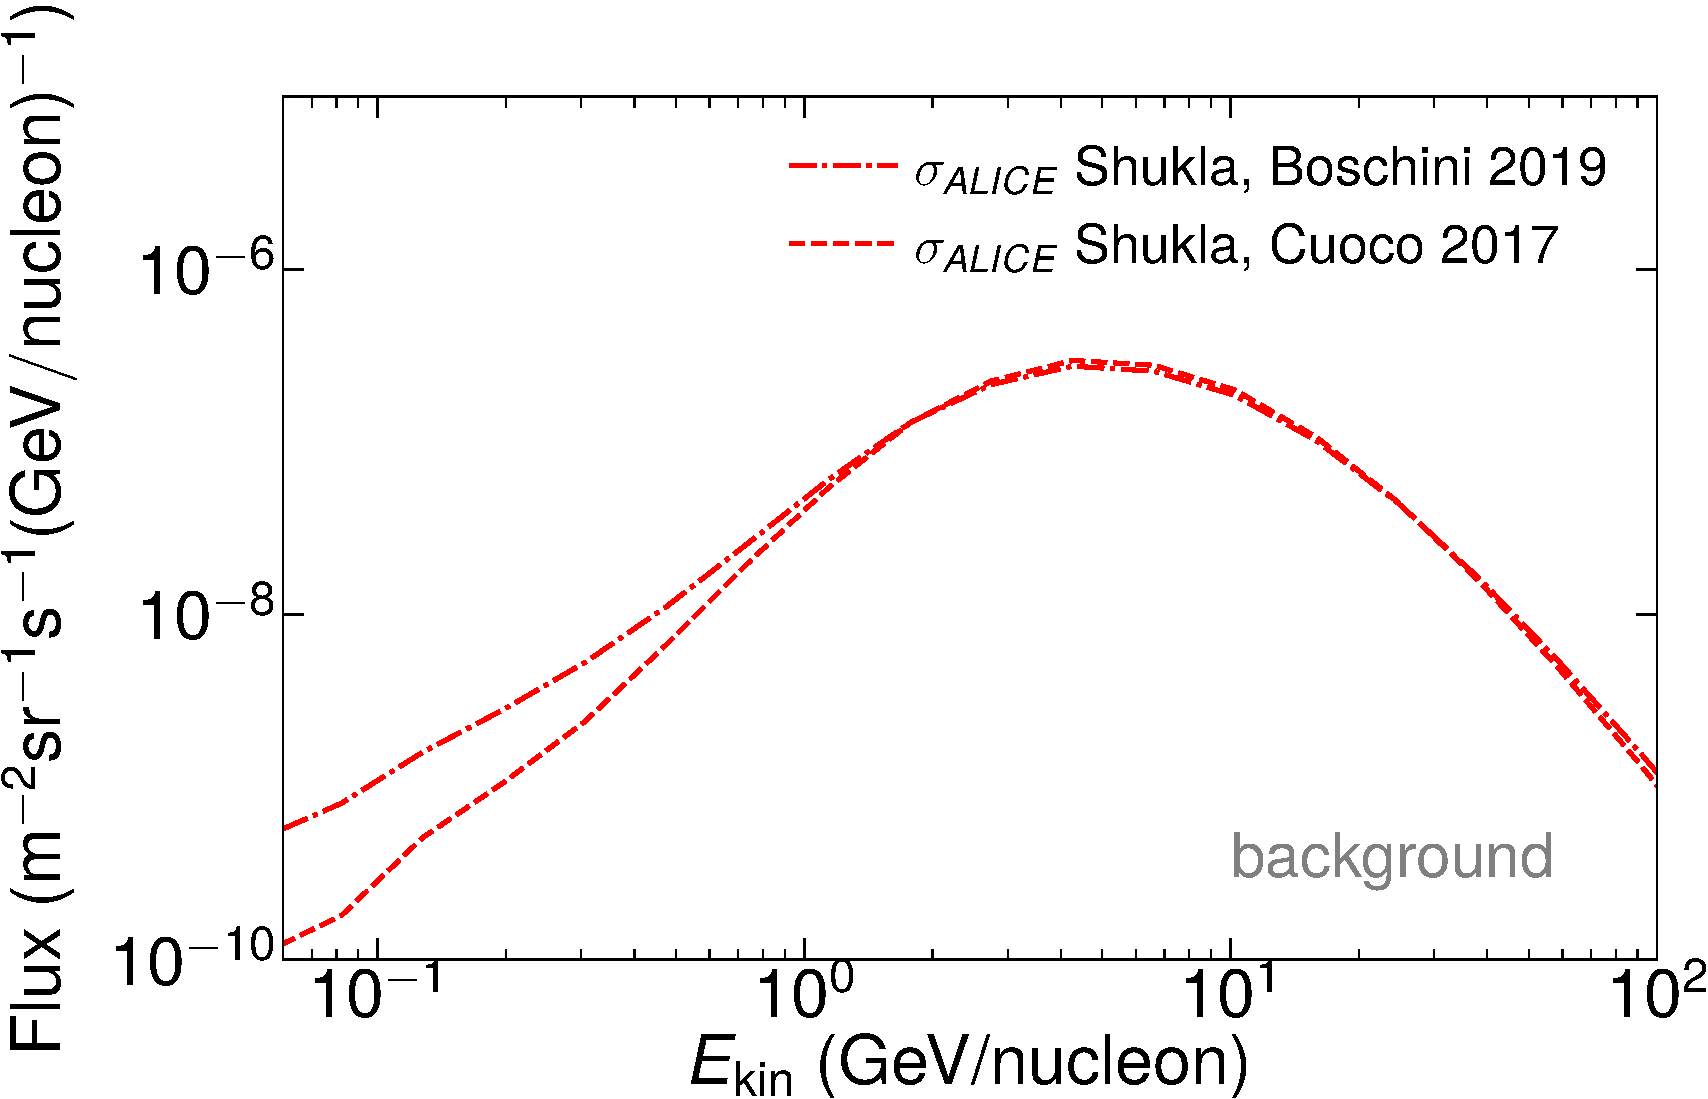
\includegraphics[width=0.45\textwidth]{figures/ComparisonPropagationBoschini.pdf}
    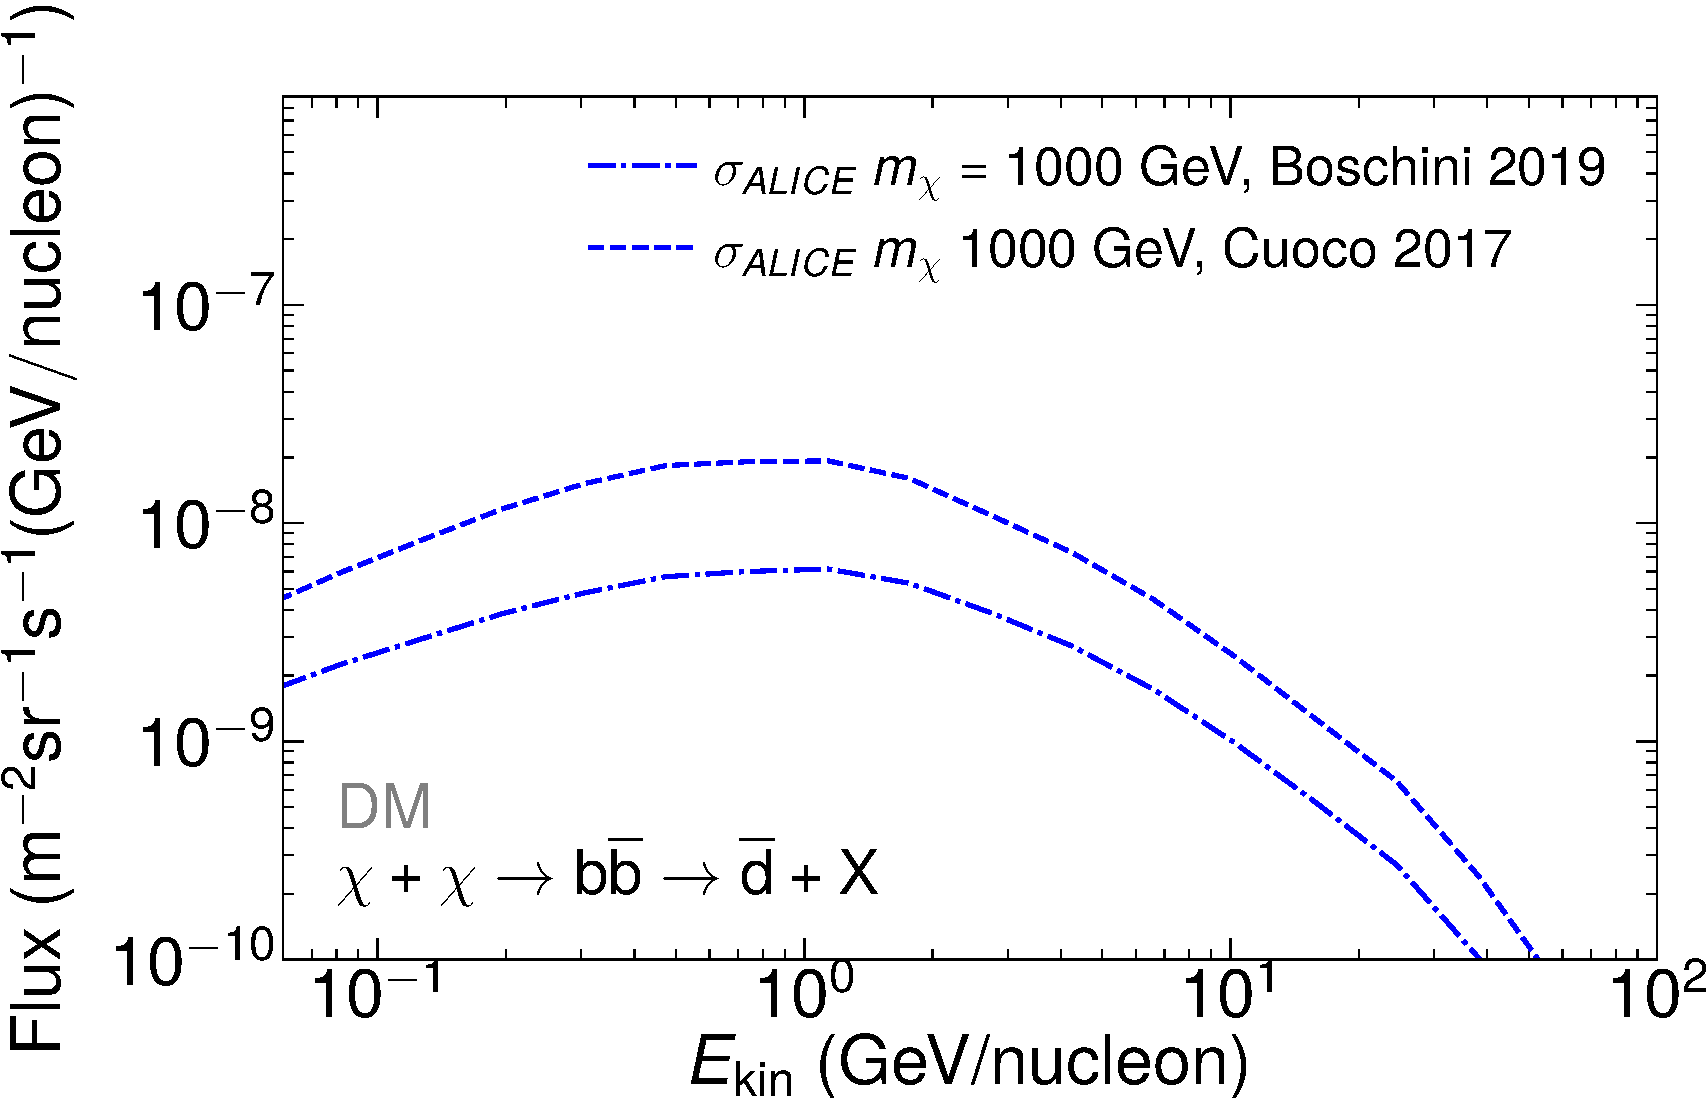
\includegraphics[width=0.45\textwidth]{figures/ComparisonPropagationBoschiniDM.pdf}
    \caption{Comparison between the different GALPROP propagation parameters used in this work, for antideuterons from high energy cosmic ray collisions (left) and from dark matter annihilations (right).}
    \label{fig:ComparisonPropagation}
\end{figure}

\subsection{The Galprop framework}\label{sec:GALPROP}
The technical details of the implementation of antinuclei propagation in GALPROP can be found in \cite{ALICE-PUBLIC-2022-002}. The following section aims to give the reader an understanding of the concepts considered.\\

As already discussed in section \ref{sec:Propagation}, the Galprop framework functions by solving the transport equation (equation \ref{eq:TransportEquation}). It does so by finding a steady state solution, iterating in smaller and smaller timesteps until a stable solution is found. During each timestep, it iterates over a position and momentum grid, the former of which can either be expressed in 2 dimensions (r and z) or 3 (x, y, z). Since we assume axial symmetry, the two are mathematically equivalent, so for the purpose of this work, the 2 dimensional method was chosen. \\

Galprop is configured by passing a set of parameters from an external text file. The important parameters are shown in table \ref{tab:GalpropParameters}. Of particular note are the Galaxy half height z$_h$, and the diffusion parameter D$_{xx}$, since these two are degenerate for cosmic rays from non-exotic sources. The actual parameter which is being fixed is the ratio of the two. This is because for non-exotic sources, the number of sources doesn't change so any change in position is compensated by increased diffusion. For a dark matter source however, the height of the galaxy has direct implications for the number of dark matter sources, so this degeneracy is broken.\\


\begin{table}[h]
    \centering
    \begin{tabular}{|c|c|c|c|}
        \hline
        Parameter &  Best fit value from Boscini & Best Fit value from Cuoco \\
        \hline
        z$_h$ &  4.2kpc & 6.2kpc \\
        \hline
        D$_{xx}$ & XX & XX \\
        \hline
    \end{tabular}
    \caption{Parameters for the tuning of Galprop. These are equivalent to the configuration of the galaxy and the propagation parameters in equation \ref{eq:TransportEquation}.}
    \label{tab:GalpropParameters}
\end{table}

It is important to note that the main parameter which a lot of propagation is the so called grammage, which is the amount of matter of the interstellar medium which particles have to traverse. This is obviously a product of the density of the interstellar medium and the path length of the particles. \\

Antinuclei are not by default included in Galprop, so in order for them to be propagated they had to be inserted into the framework. Fortunately, the framework is capable of handling negative nuclei with antiprotons, therefore the extension was done by providing the mass of the antideuteron/antihelium, their inelastic cross sections on the interstellar medium, and their source functions. Separate entries were used for the secondary production from high energy cosmic rays and from dark matter annihilations. The inelastic cross section had to be provided on a proton and helium target, which are significantly lighter than the average detector materials probed in the measurements shown in section \ref{sec:ResHe3SigmaInel}, therefore the results had to be extrapolated to these lighter targets. The exact methods of the extrapolations are explained in section \ref{sec:ResAnnInOurGalaxy}.\\

The source functions for antinuclei from either high energy cosmic ray collisions or from dark matter annihilations were included in the GALPROP as a function of the distance from the galactic centre. For the dark matter part, this can be done simply by evaluating the equation described above for a specific radius and kinetic energy. However, for antinuclei from high energy cosmic rays this is not possible, since the spectrum of cosmic rays at a given point enters into the equation. Therefore, PLEACEHOLDER FOR TEXT EXPLAINING THE IMPLMENTATION OF THE SECONDARIES.
%To do : 2 paragraphs on the implenetation of secondaries
\subsection{Annihilations within our galaxy}\label{sec:ResAnnInOurGalaxy}
As antinuclei travel through our galaxy, they will interact with matter in the interstellar medium and might interact inelastically. This can either be in the form of inelastic scattering or annihilation, although of the two the latter is expected to be dominant \cite{}. The result of these interaction is thus mostly the disappearance of the antinuclei. The produced particles are mostly pions, and thus not stable enough to detect them and maybe extract a signal from them. Some high energy photons could also be produced, and such gamma rays are the target of specific sky surveys looking for large areas of antimatter, which when coming into contact with matter should produce a detectable signal. However, a single annihilation would be undetectable at any significant distance. We can therefore conclude that the relevant result of annihilation is the disappearance of the antinucleus in question. \\

This process was implemented in galprop by implementing an inelastic cross section. As antinuclei are propagated throughout our galaxy, the total amount of matter they interact with is calculated for each momentum step. In order to do so, both the distribution and the makeup of the interstellar is required. The makeup is known to a relatively high accuracy \cite{}, and is dominated by hydrogen, which makes up $\approx$90\% of the total mass in the interstellar medium. The remainder is mainly helium, making up $\approx 9\%$ of the total mass. During each calculation step, the inelastic cross sections on the dominant species of the interstellar medium (hydrogen and helium) are used to calculate how many antinuclei are lost in each momentum bin. Therefore, it is necessary to evaluate the cross sections on these very light targets, rather than the heavy targets on which they were measured.\\

In order to extrapolate, the general shape of the antinucleus-proton cross section in Geant4 was modified by the measured deviation from the antinucleus-target cross section reported in sections \ref{sec:ResHe3SigmaInel}, \ref{sec:ResTritonSigmaInel} and in \cite{}. This assumes that the relative scaling is the same regardless of the target nucleus, although an additional 8\% uncertainty is assigned to allow for any deviation from this assumption. For values outside the range of the measurements detailed in sections \ref{sec:ResHe3SigmaInel}, the scaling factor at the last available momentum was used.
The resulting cross sections are shown for both antideuterons and \ahe\ in figure \ref{fig:ScaledXS_ahe_adeut}. 

\begin{figure}
    \centering
    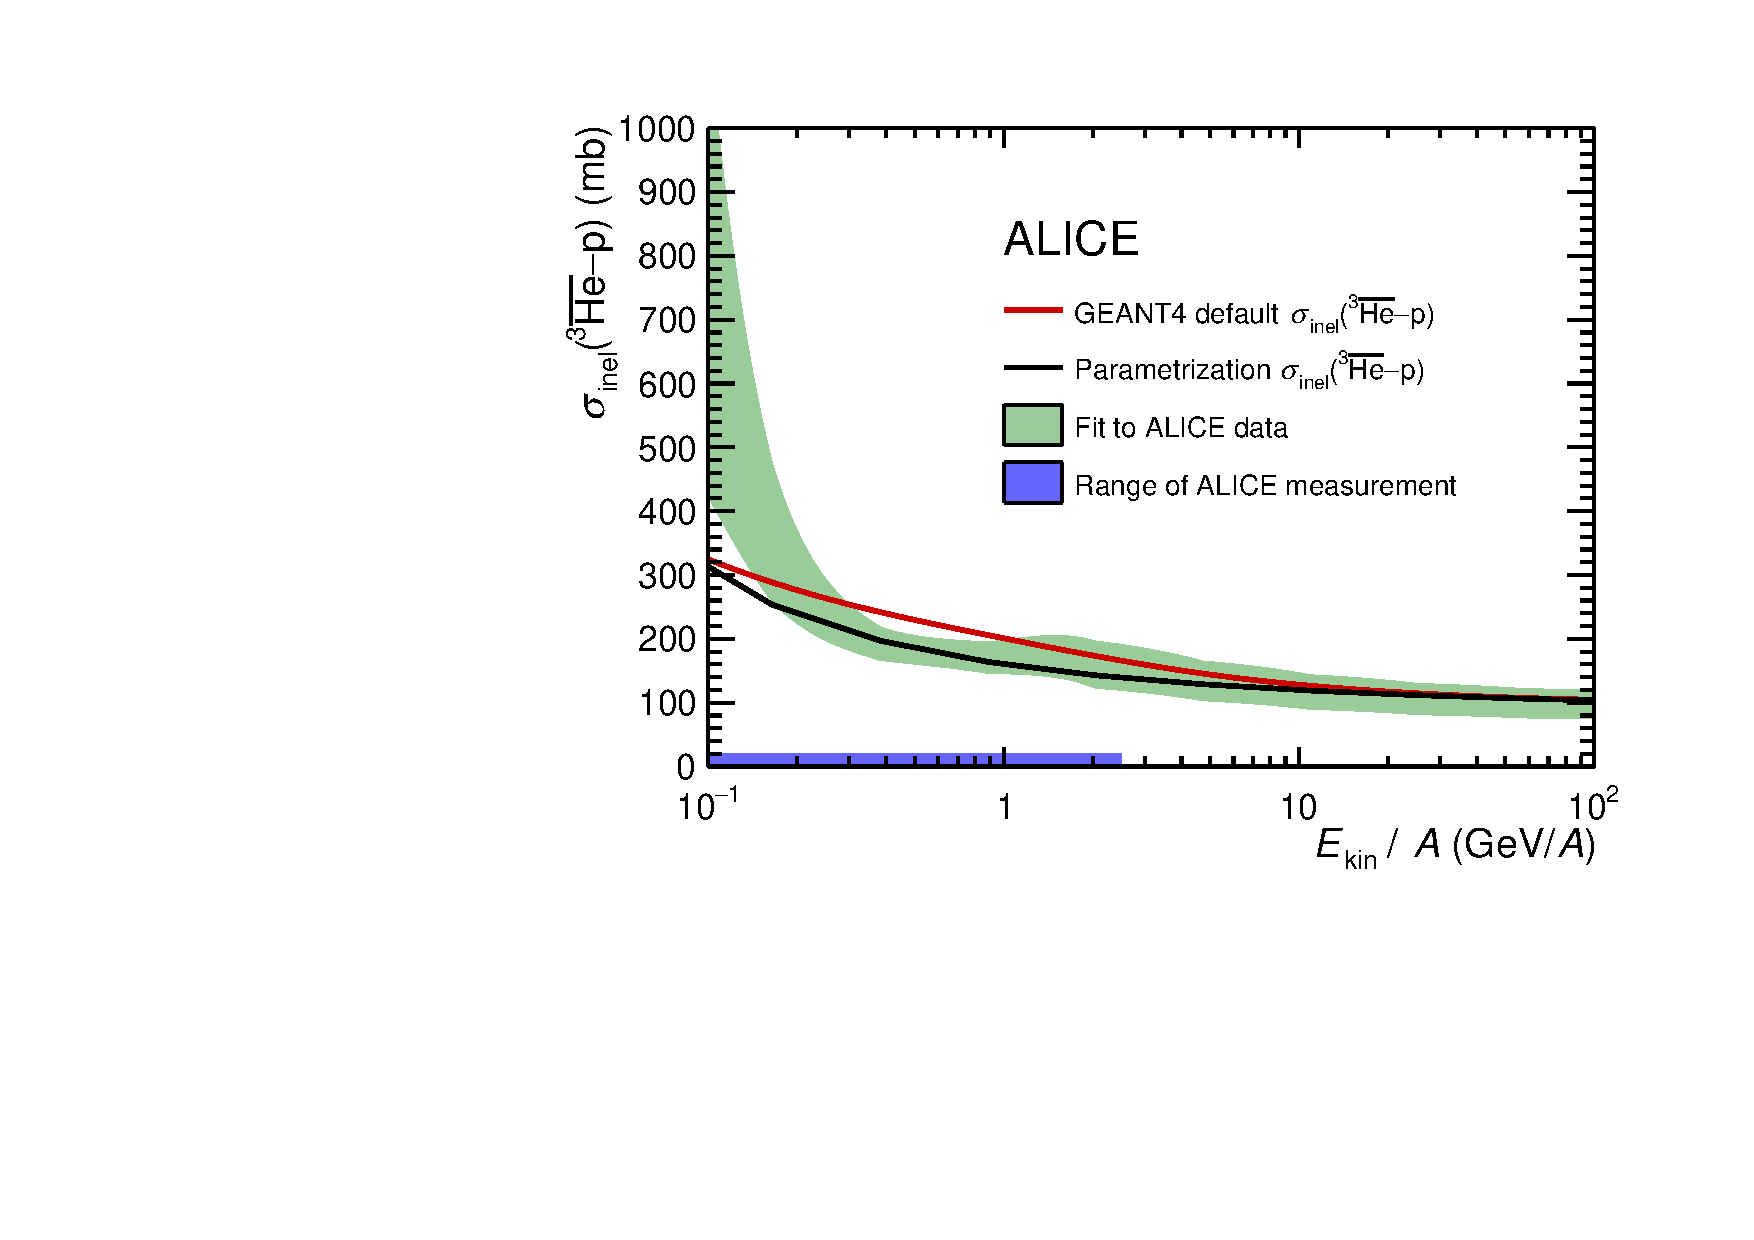
\includegraphics[width=0.45\textwidth]{figures/Antihelum_on_p_targets_scaled_with_paramterisation.pdf}
    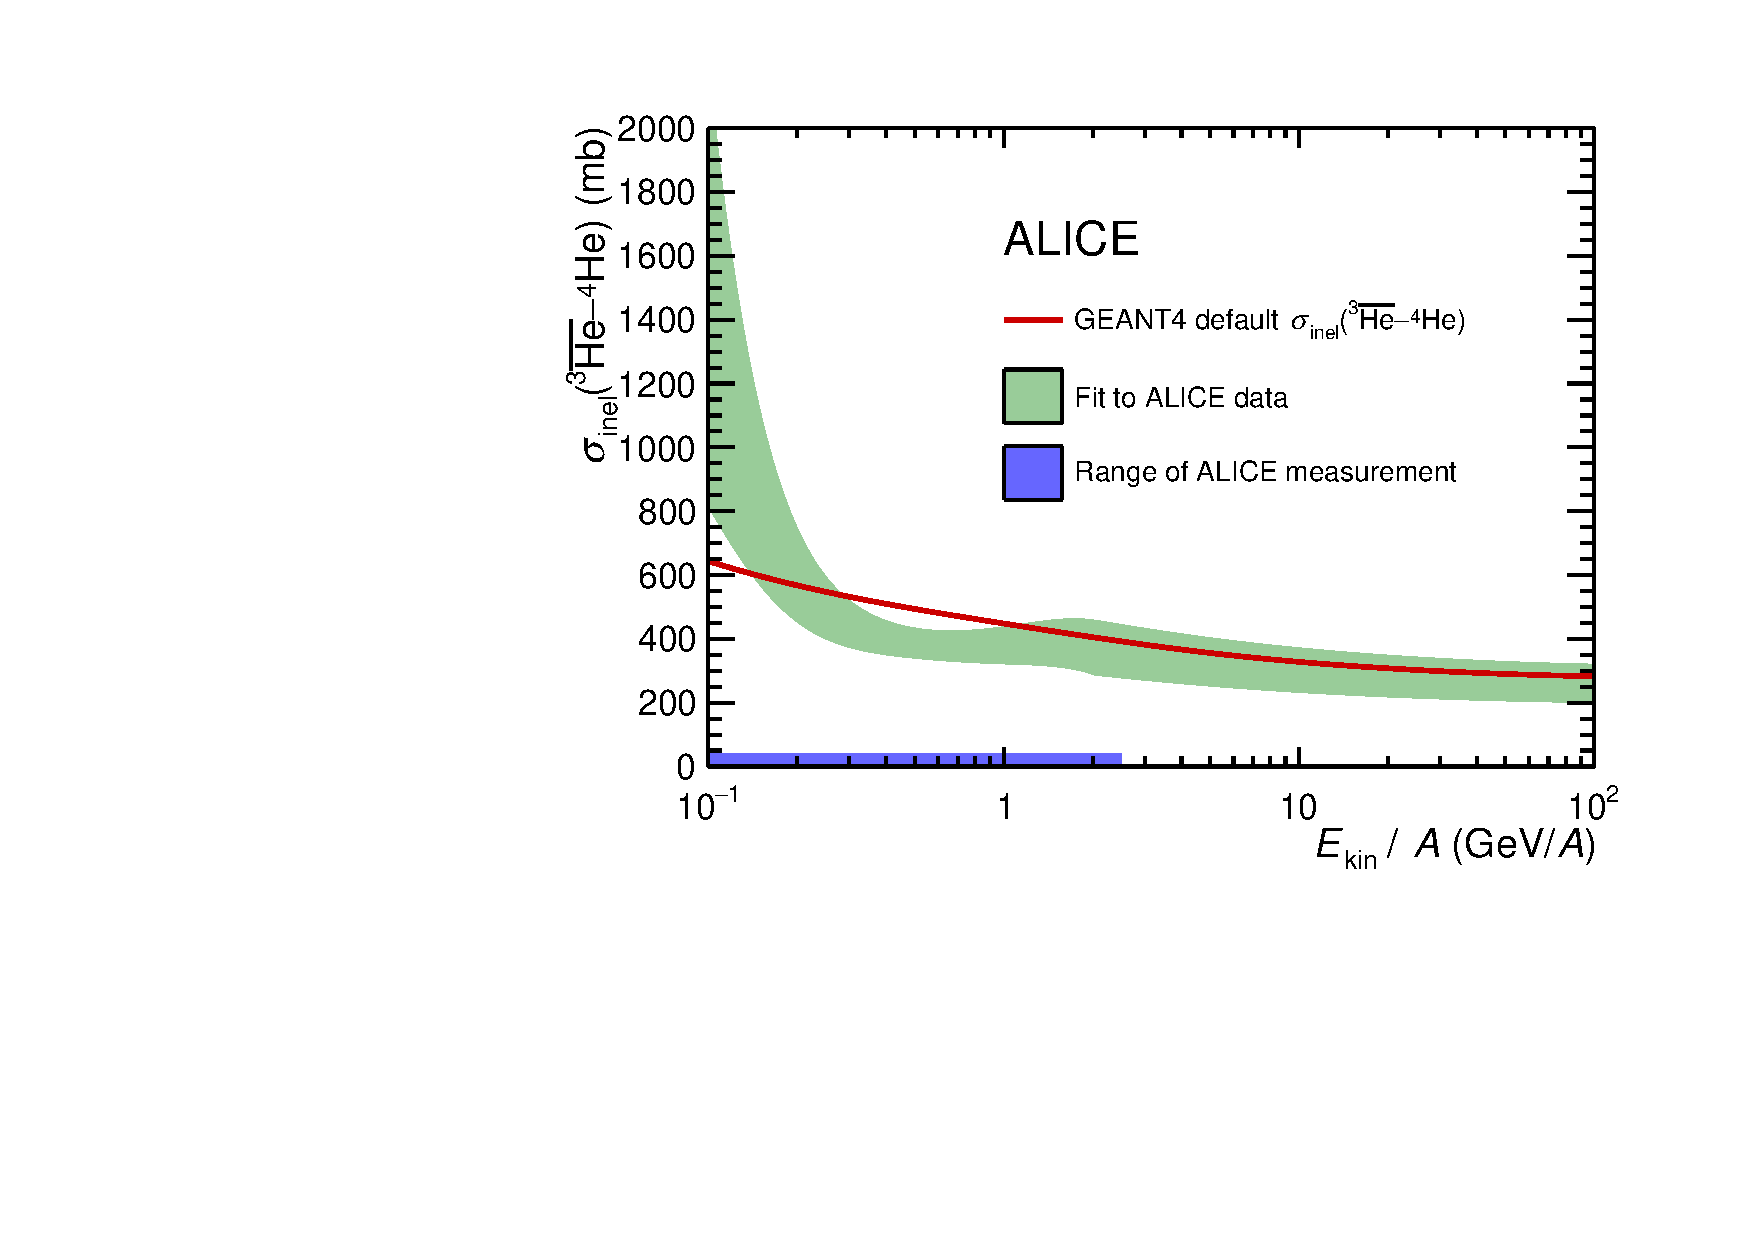
\includegraphics[width=0.45\textwidth]{figures/Antihelum_on_p_targets_scaled.pdf}
     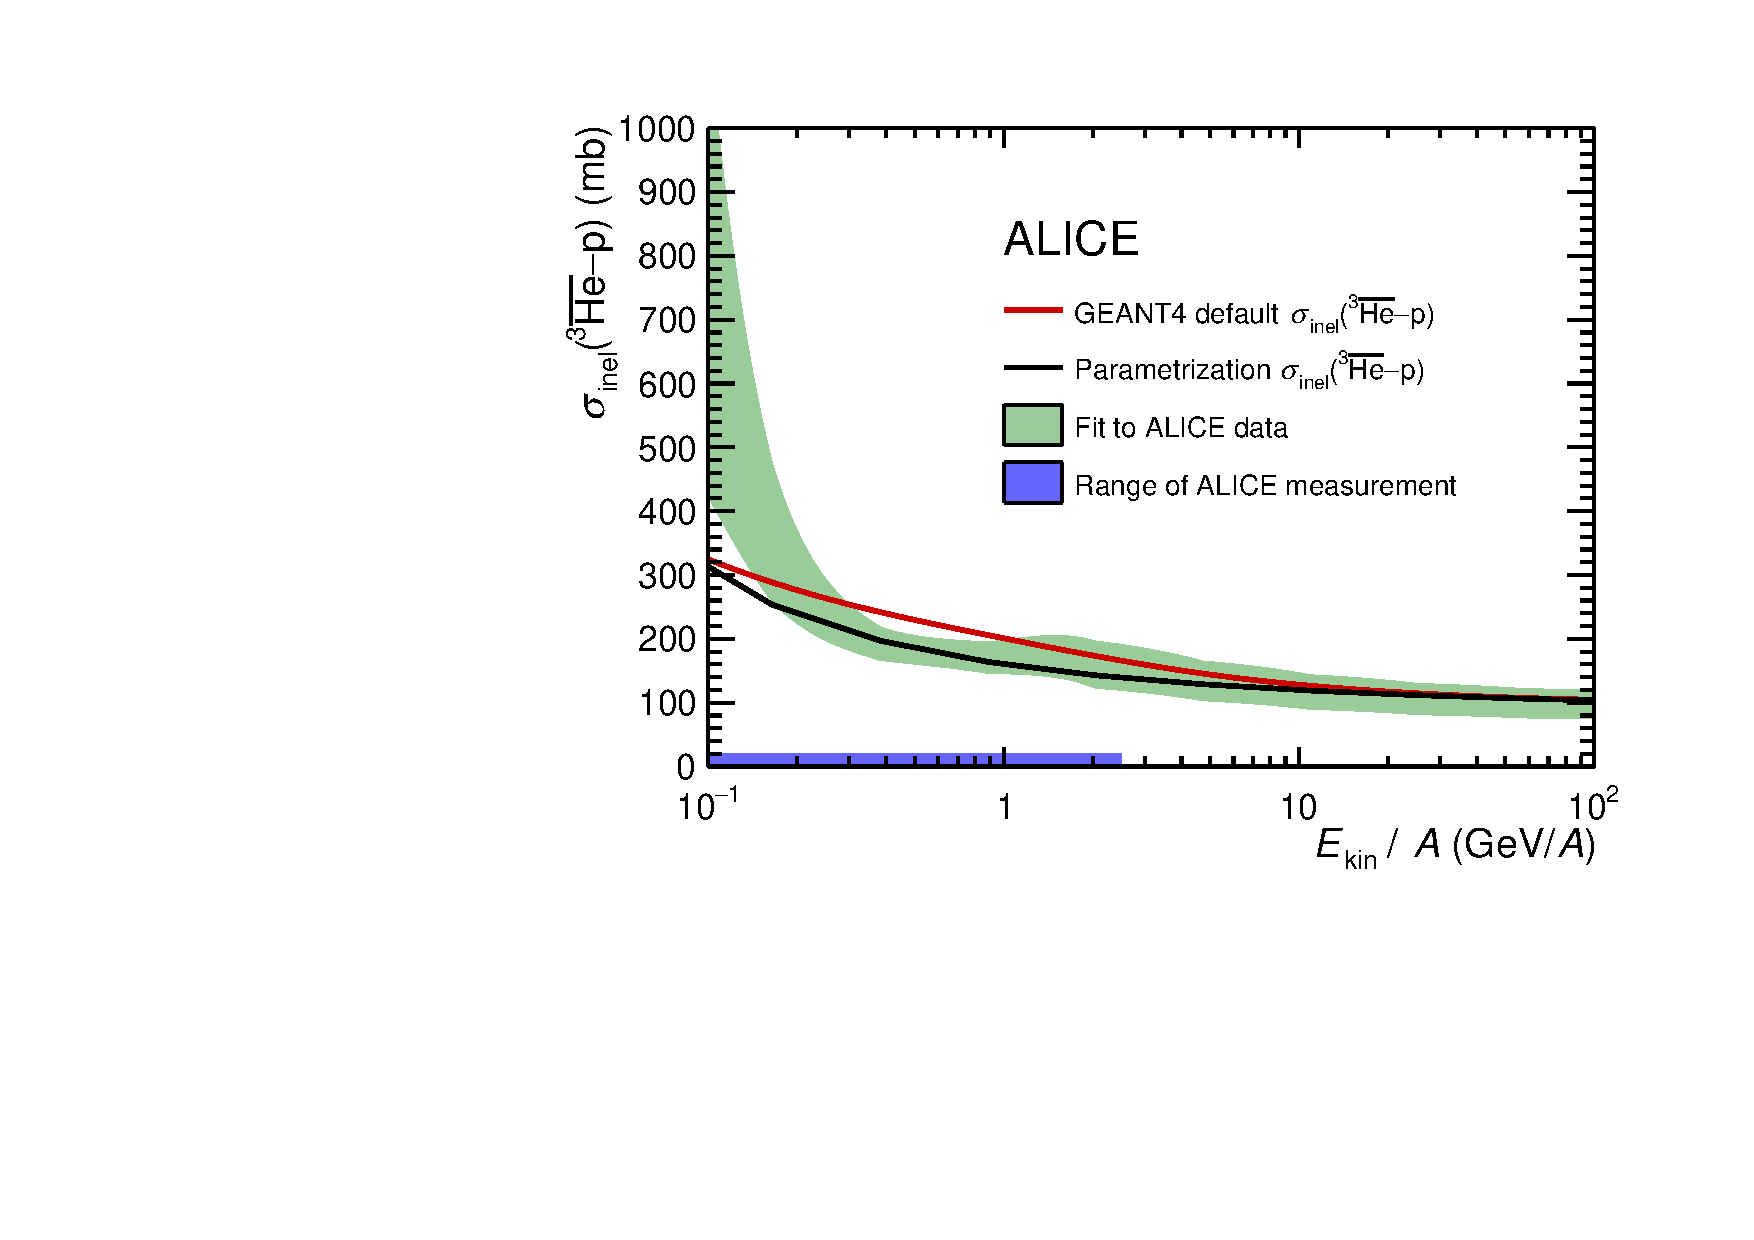
\includegraphics[width=0.45\textwidth]{figures/Antihelum_on_p_targets_scaled_with_paramterisation.pdf}
    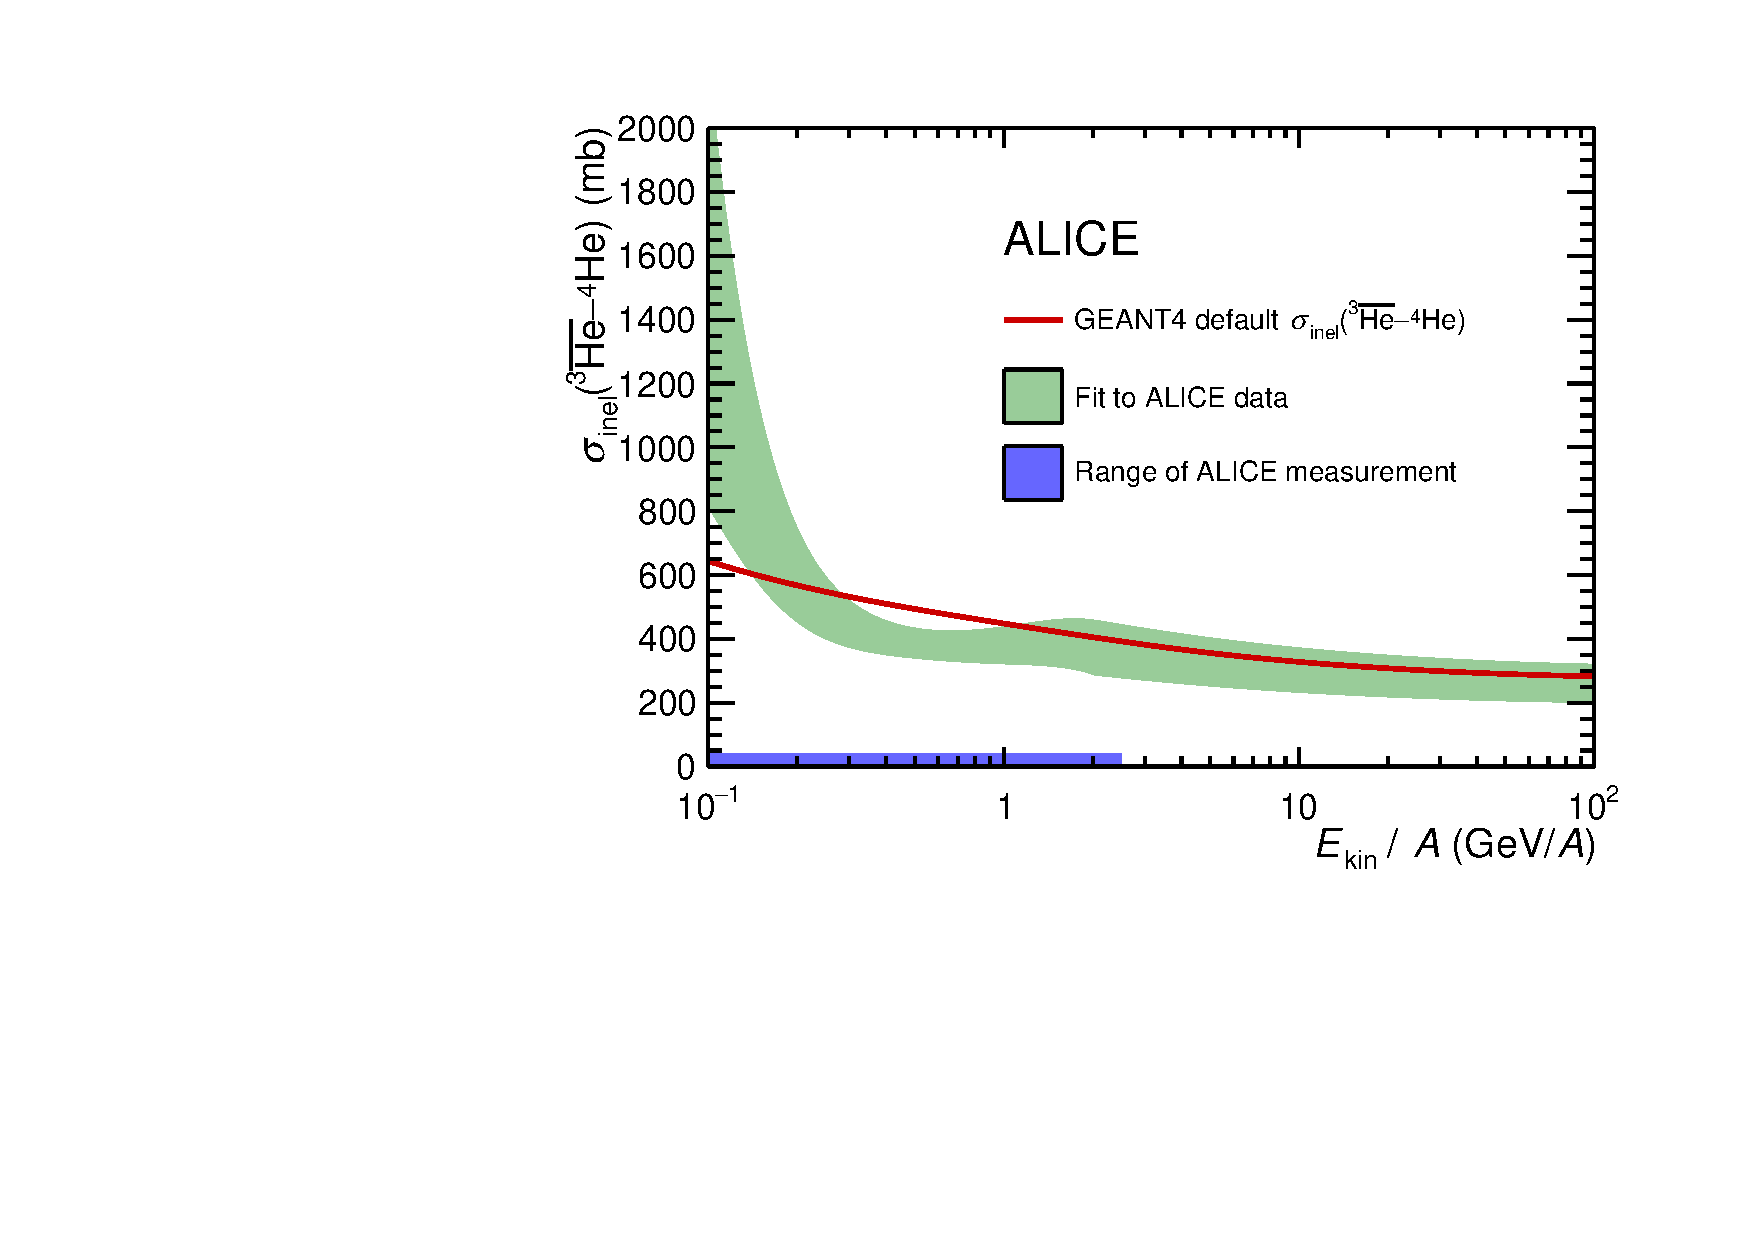
\includegraphics[width=0.45\textwidth]{figures/Antihelum_on_p_targets_scaled.pdf}
    \caption{Scaled inelastic cross sections of \ahe\ (top) and antideuterons (bottom) on proton (left) and Helium-4 (right) targets. The band shows the experimental uncertainty from the ALICE measurements \cite{}, plus an additional 8\% uncertainty associated with the scaling from heavier targets (C, O, Al) to protons (H).}
    \label{fig:ScaledXS_ahe_adeut}
\end{figure}


\subsection{Results for antideuterons}
Presented in this section are the results for the effect of different dark matter profiles and masses on the expected antideuteron fluxes from dark matter. They are also compared to secondary antideuterons produced in high energy cosmic ray collisions with the interstellar medium. 

\subsubsection{Results for different dark matter masses}
In this section the effects of different dark matter masses on the antideuteron fluxes will be discussed. The fluxes can be found in figure \ref{fig:Results_dbar_fluxes_diff_DM_masses}, where they are compared to a prediction for secondary antinuclei from high energy cosmic ray collisions with the interstellar medium. In the lower panel on each figure, the transparency of the galaxy to antideuterons is shown. This is defined in equation \ref{eq:TransparencyDefinition} as the ratio of the obtained flux with a given parameterization of the inelastic cross section, to the flux obtained when all inelastic interactions are set to zero.

\begin{equation}\label{eq:TransparencyDefinition}
    \mathrm{Transparency(sigma_{inel})} = \frac{\mathrm{Flux(sigma_{inel}})}{\mathrm{Flux(sigma_{inel}=0})} 
\end{equation}

\begin{figure}
    \centering
    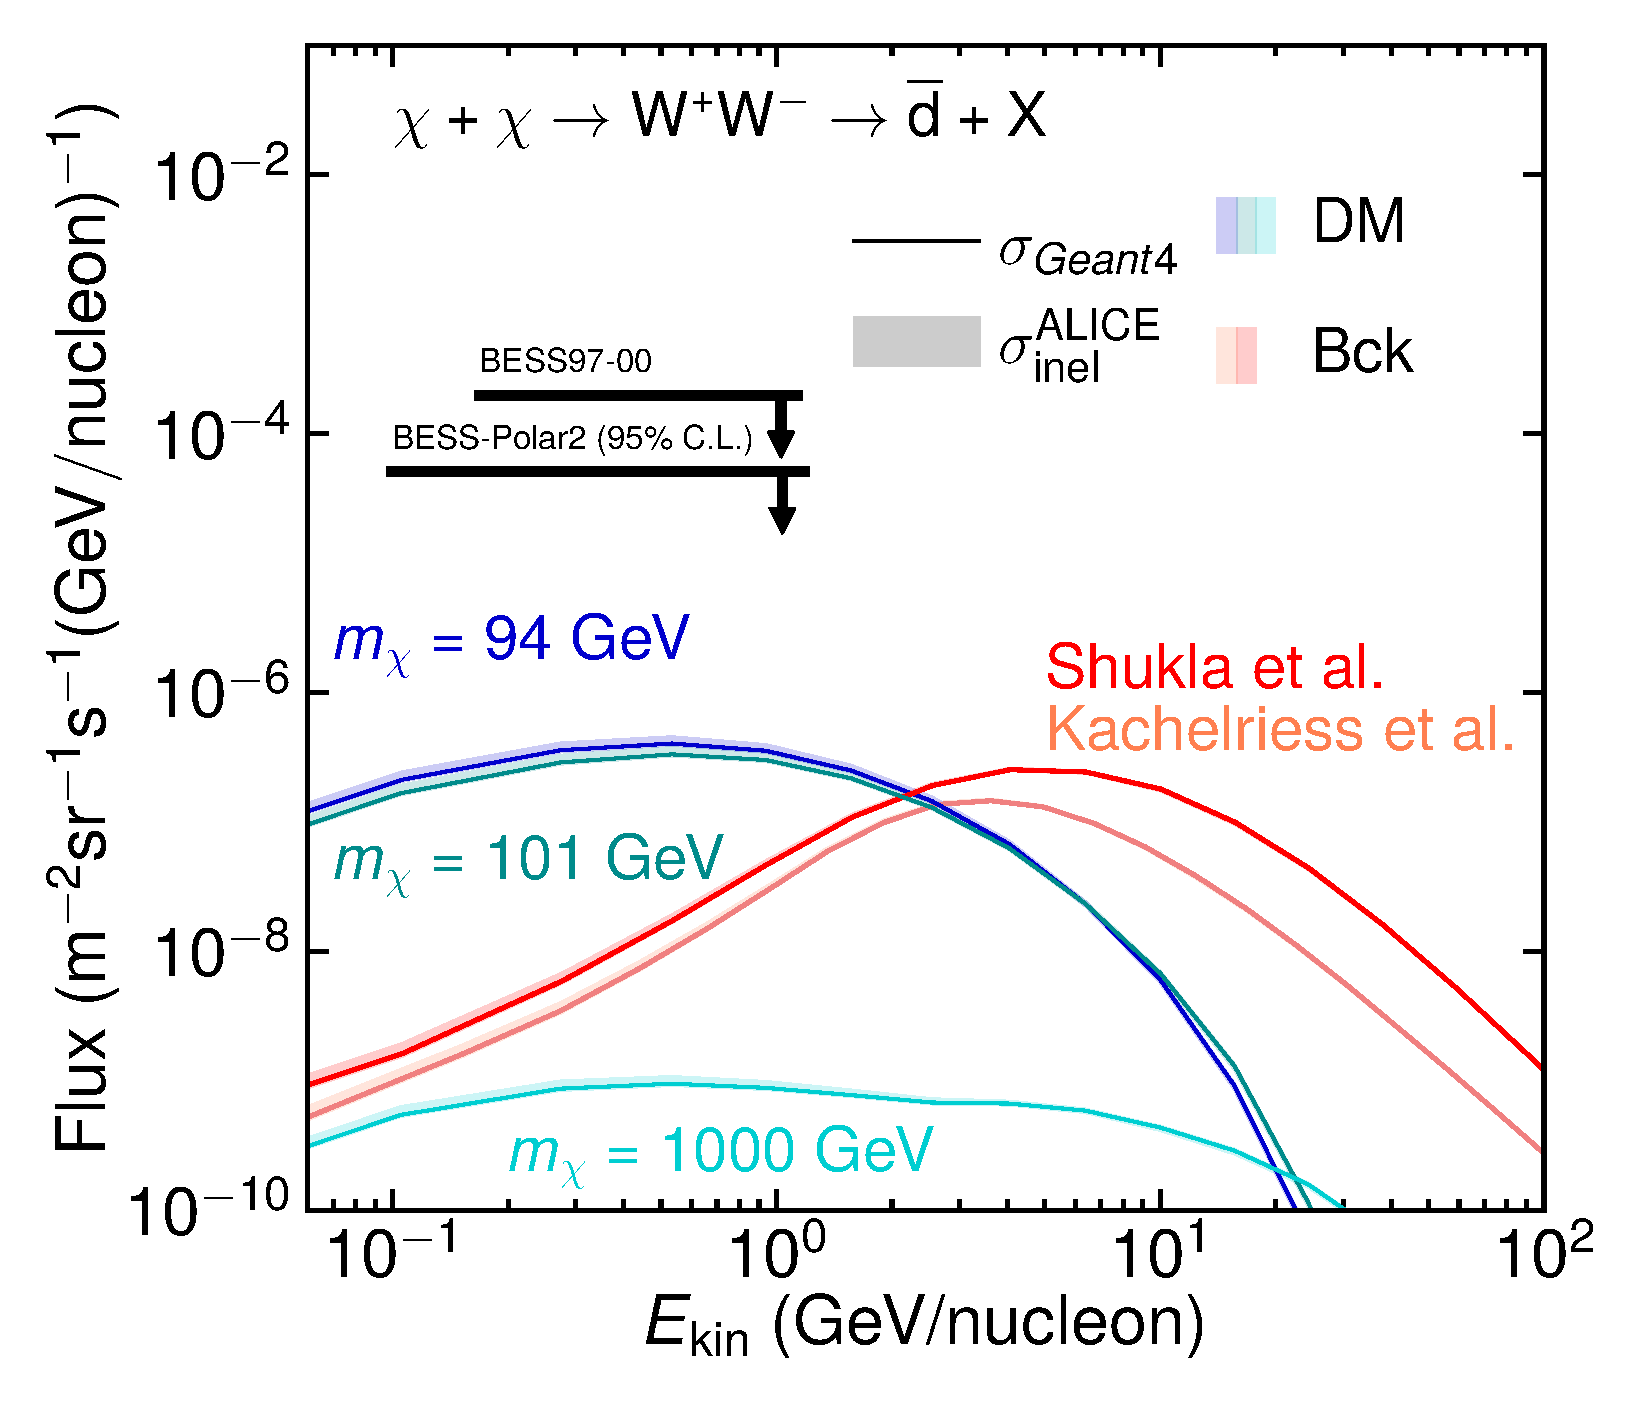
\includegraphics[width=0.45\textwidth]{figures/WWdbarPaperTOA.pdf}
    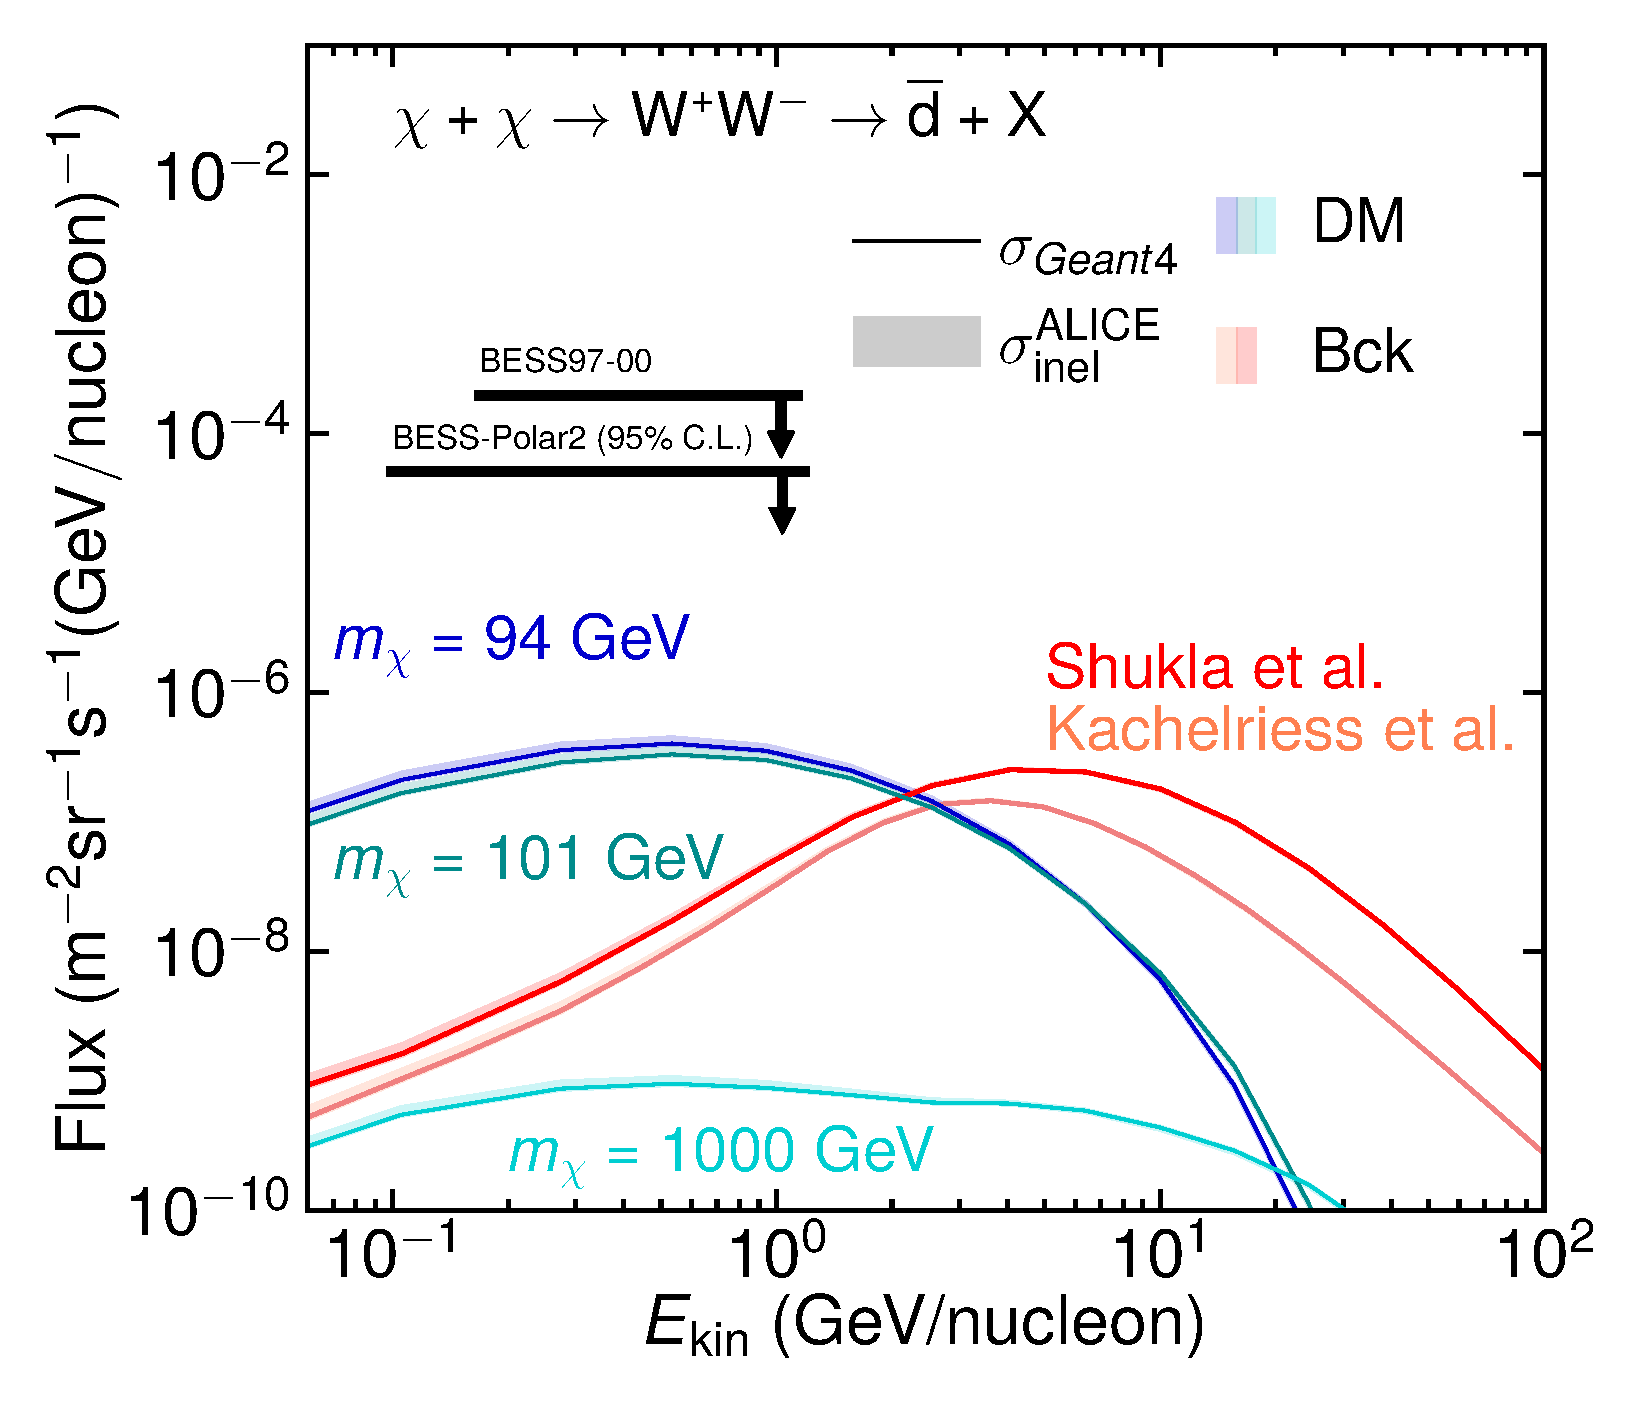
\includegraphics[width=0.45\textwidth]{figures/WWdbarPaperTOA.pdf}
    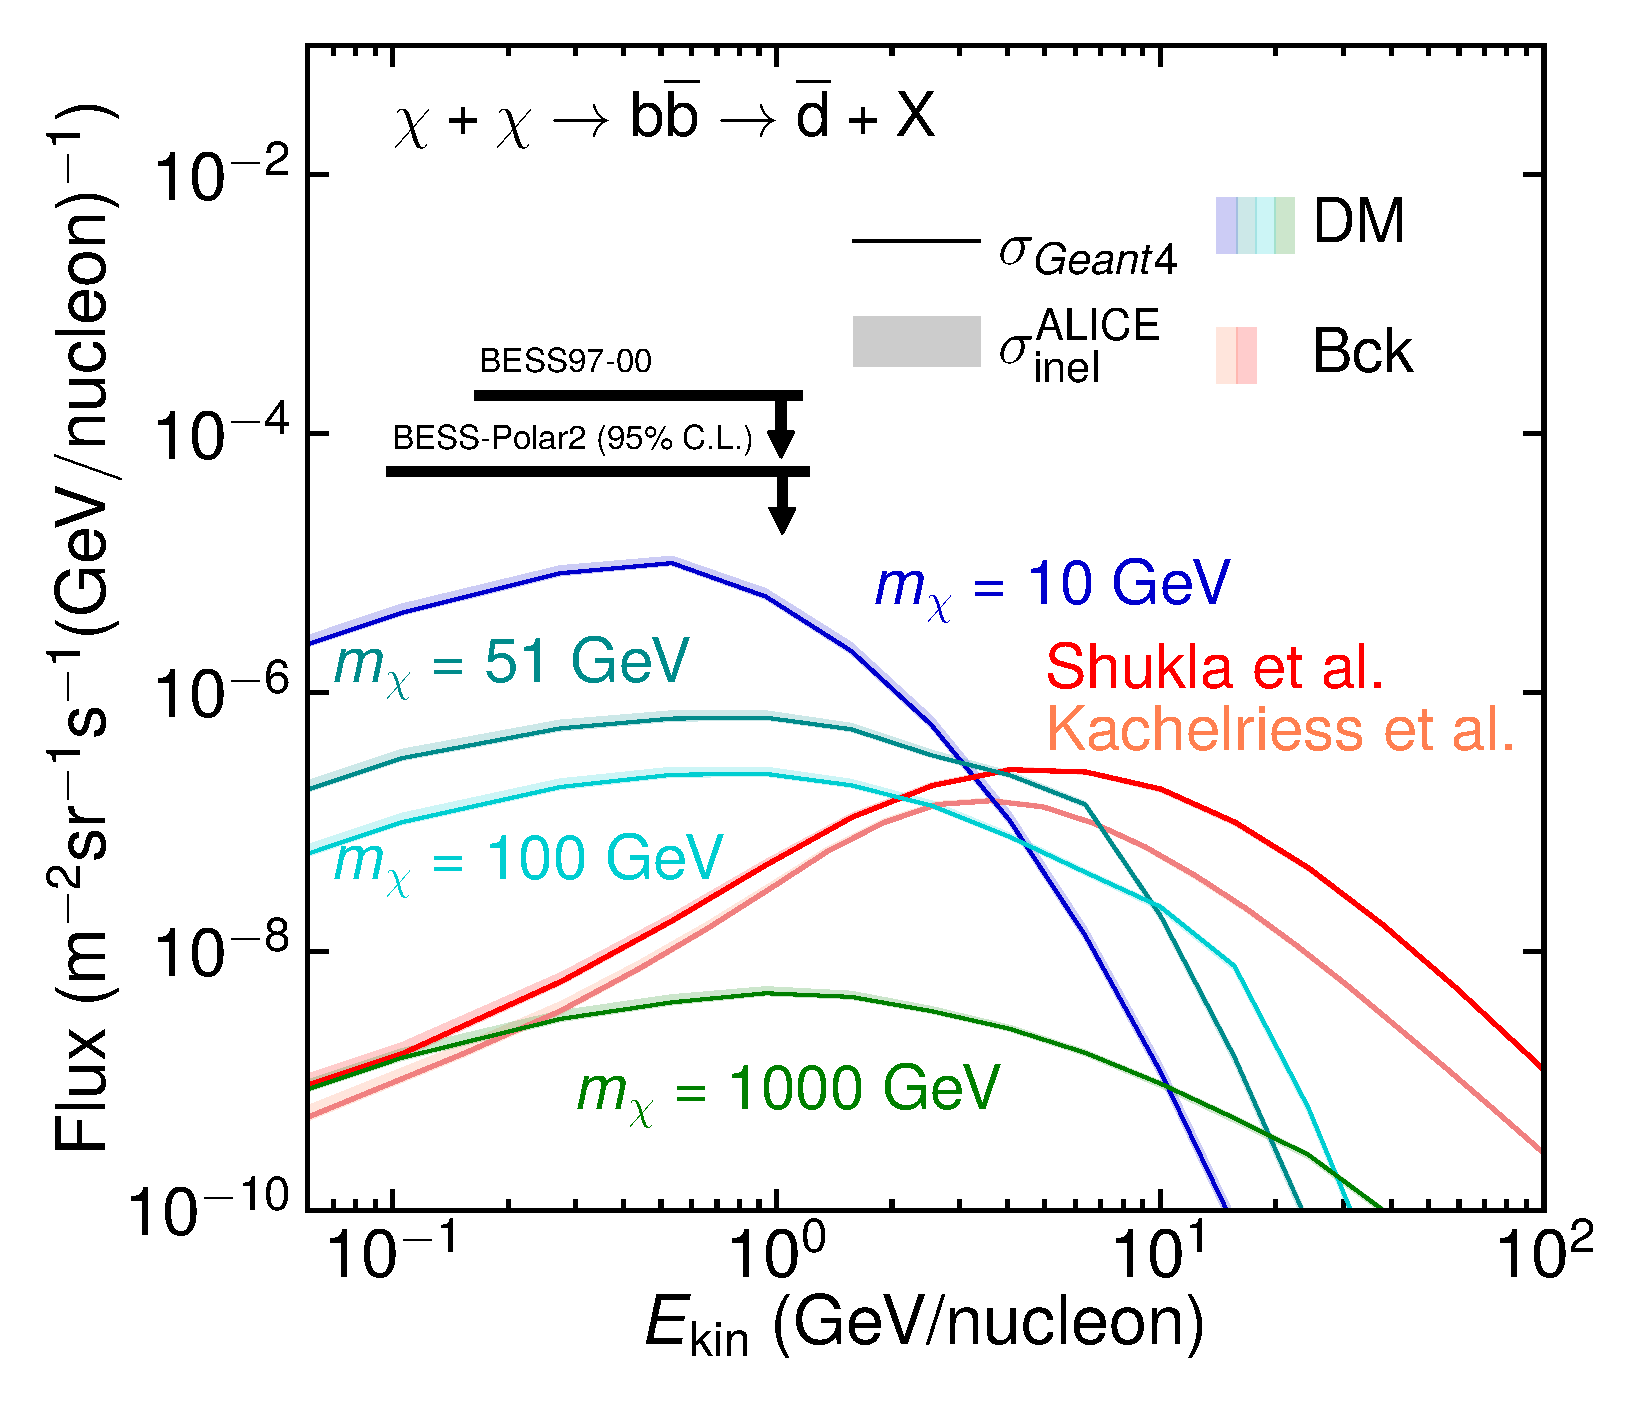
\includegraphics[width=0.45\textwidth]{figures/bbdbarPaperTOA.pdf}
    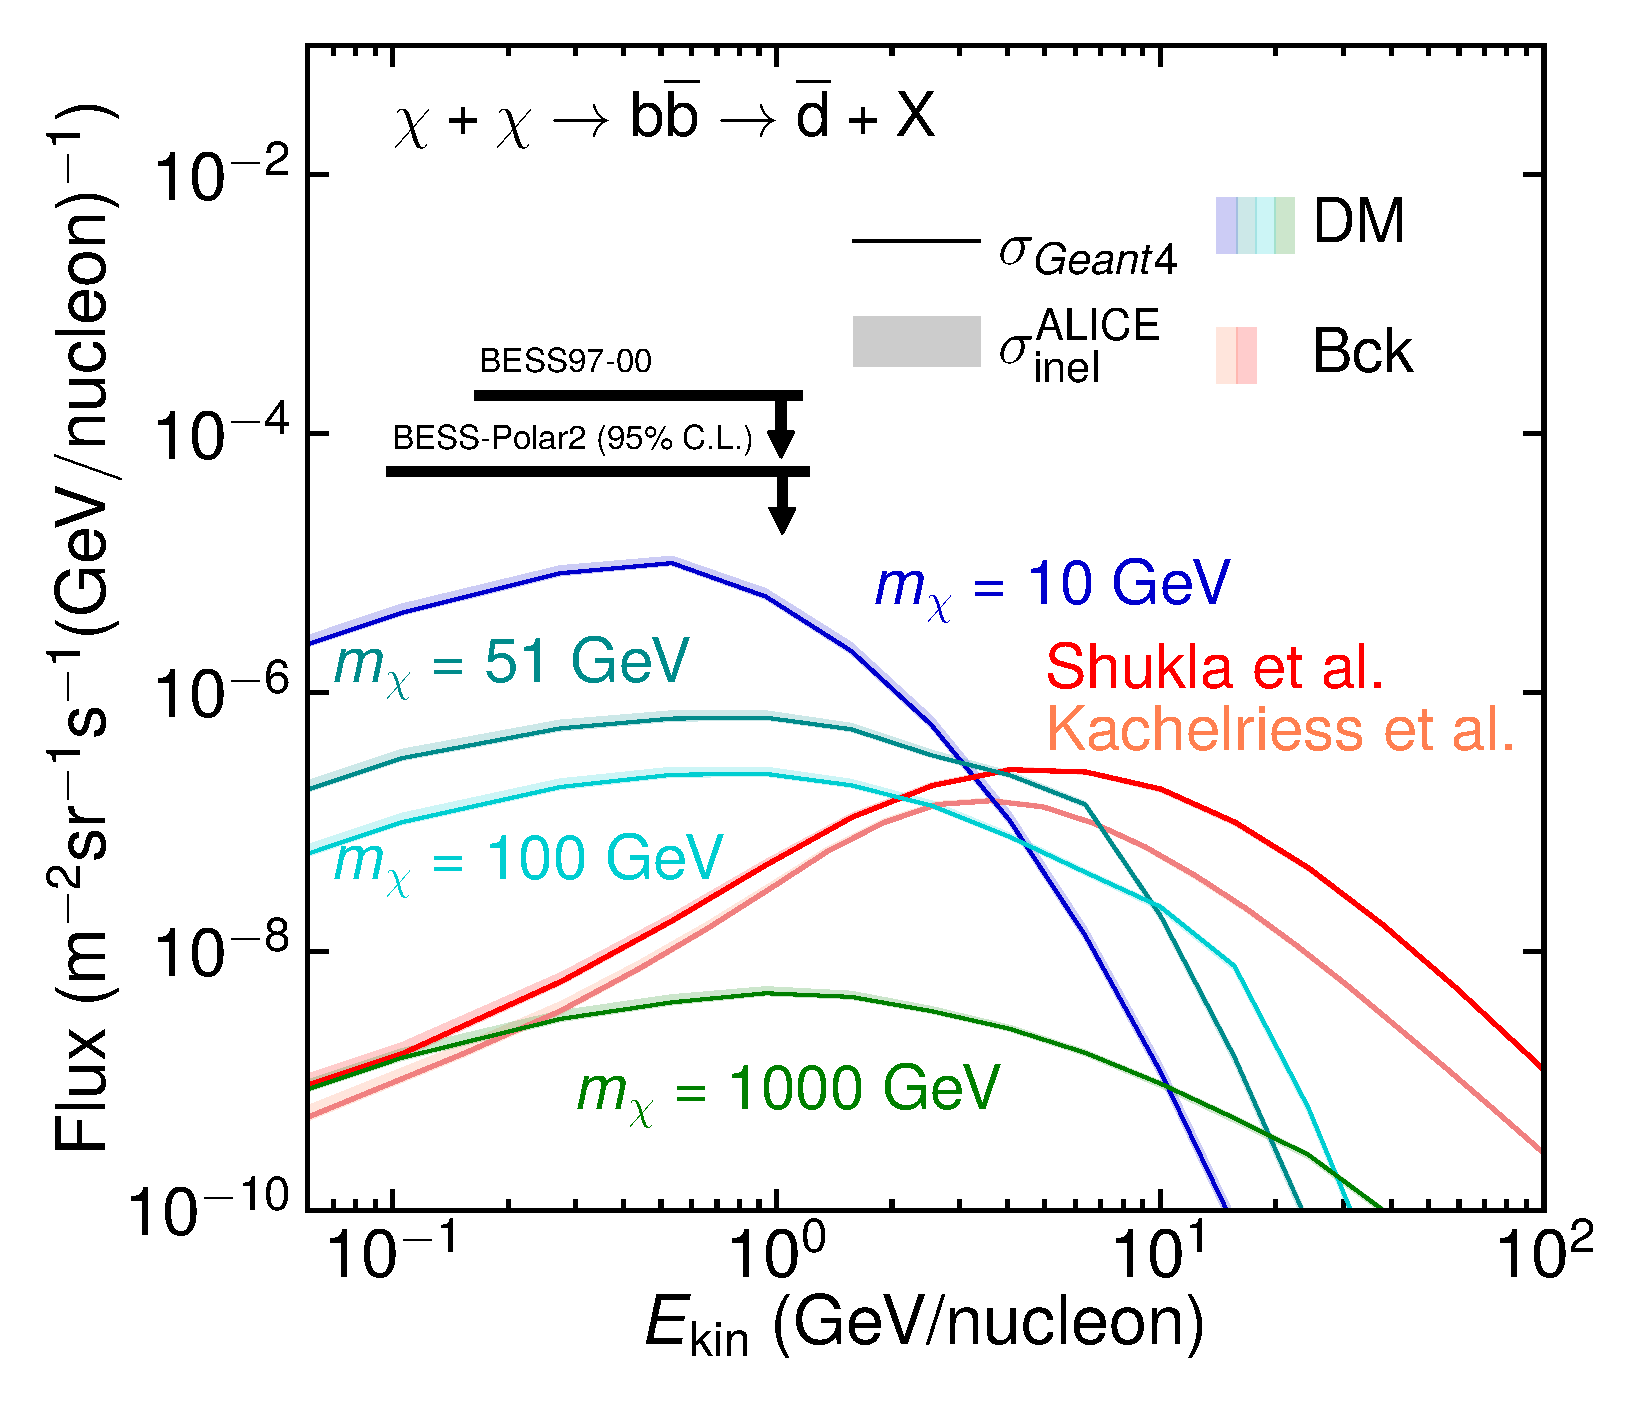
\includegraphics[width=0.45\textwidth]{figures/bbdbarPaperTOA.pdf}
    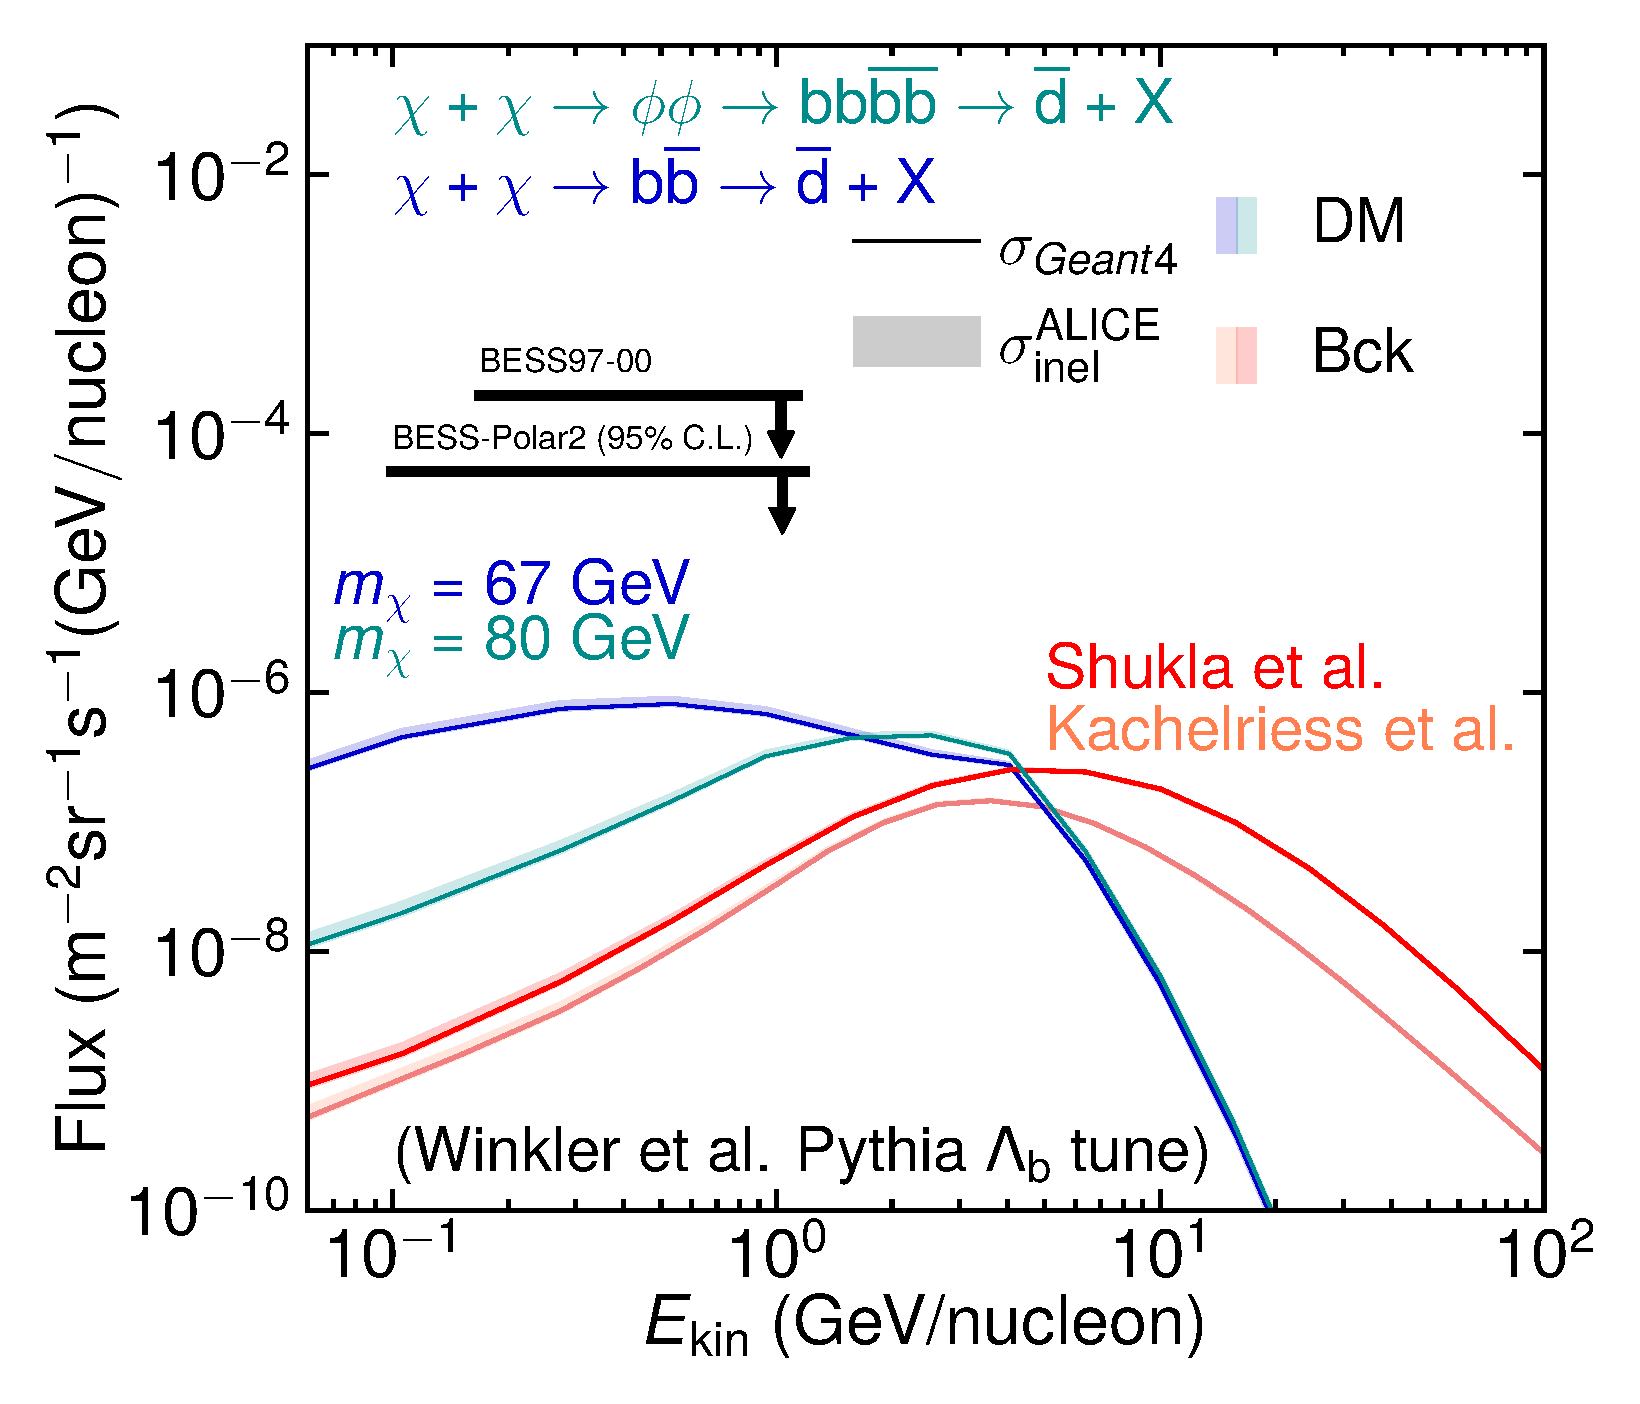
\includegraphics[width=0.45\textwidth]{figures/blambdadbarPaperTOA.pdf}
    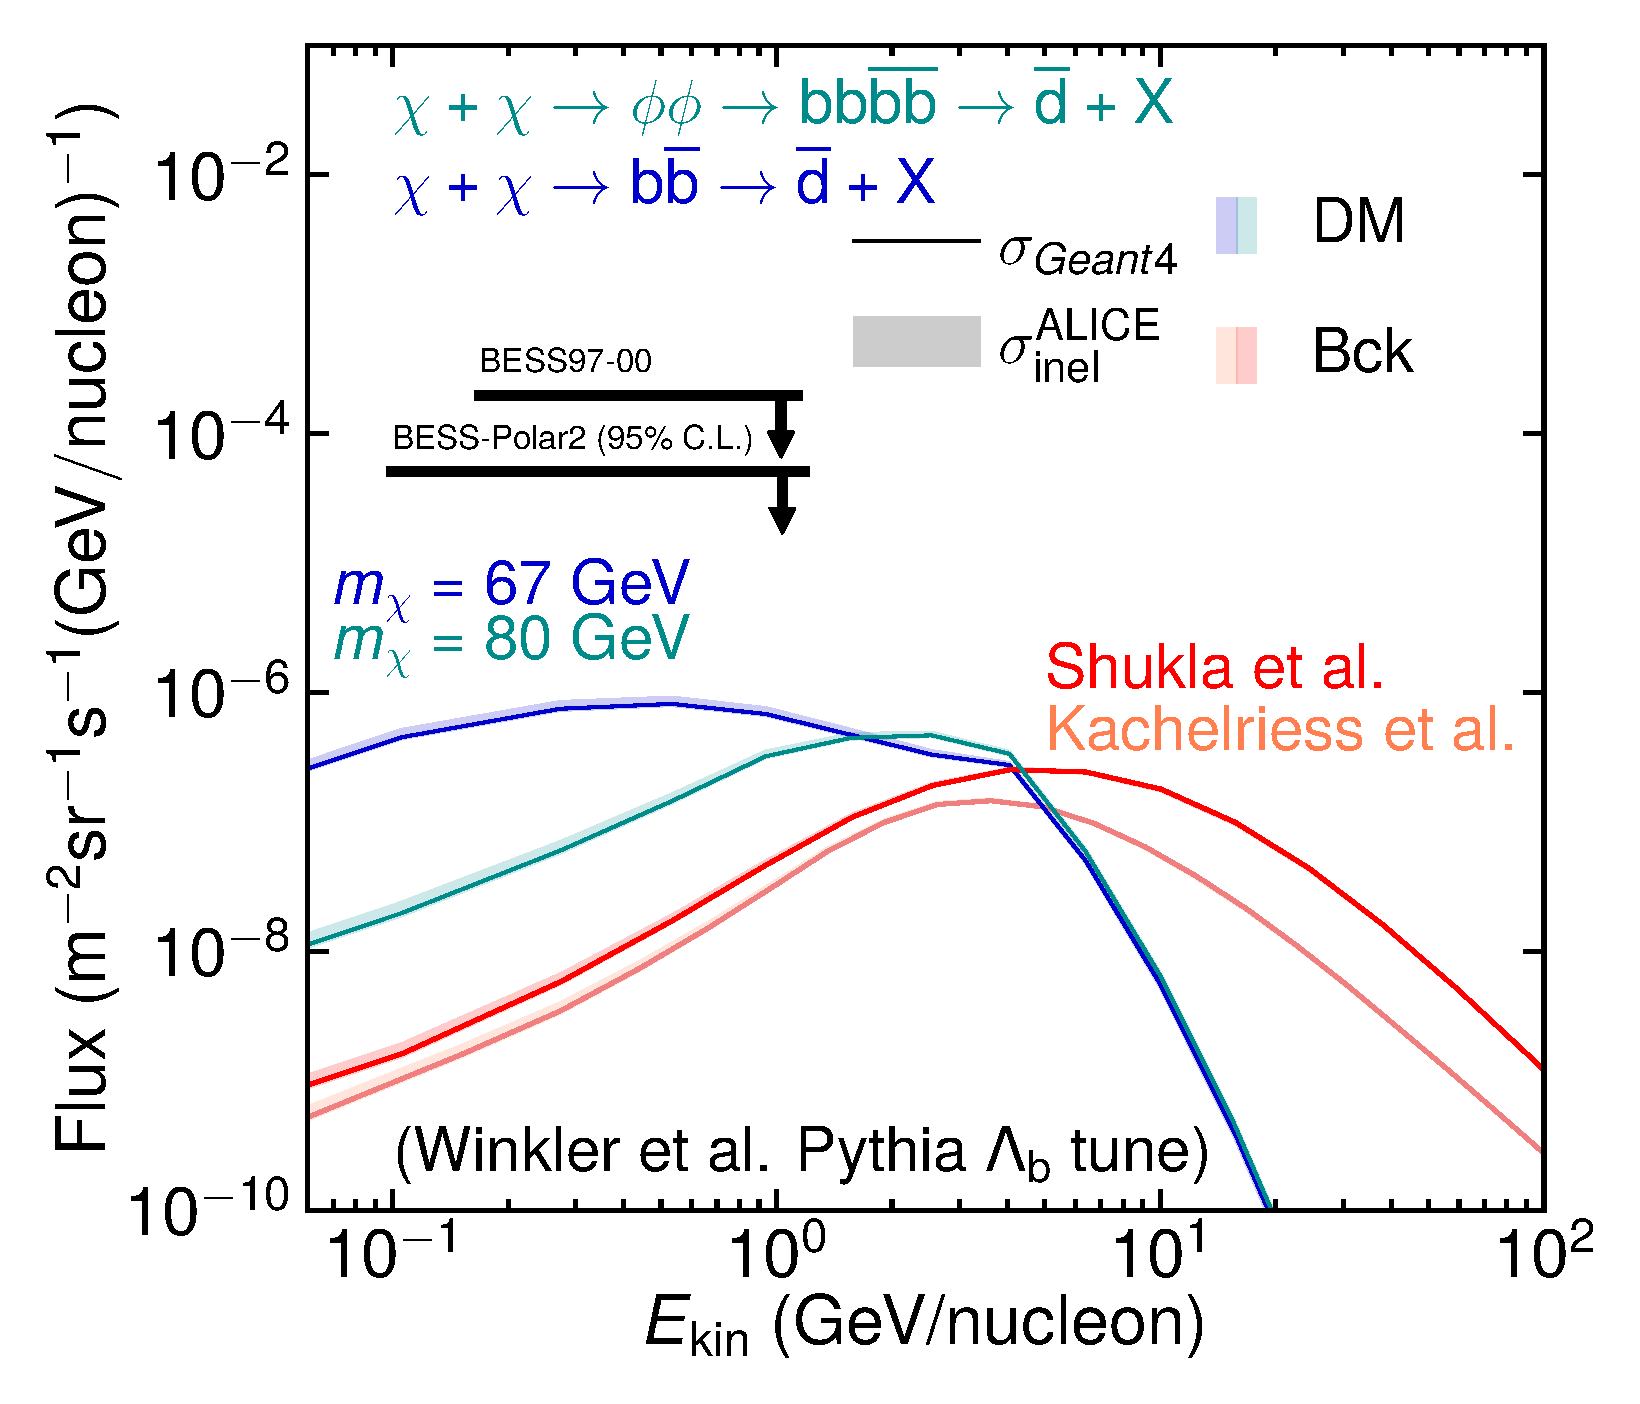
\includegraphics[width=0.45\textwidth]{figures/blambdadbarPaperTOA.pdf}
    \caption{Expected antideuteron fluxes for different \dmm\ ranging from 51GeV to 1TeV. They are compared to an expected spectrum of secondary antideuterons from high energy cosmic ray collisions. The results are shown for the position of the solar system. The figures on the left show the results without solar modulation, and on the right with solar modulation included by means of a force field model, as is discussed in section \ref{sec:Propagation}. The results are also shown for different possible annihilation channels of dark matter, either through \WW\ (top), through \bb\ (middle) or through $\Lambda_b \rightarrow $\bb and light mediators (bottom).}
    \label{fig:Results_dbar_fluxes_diff_DM_masses}
\end{figure}


\subsubsection{Results for different dark matter profiles}


\subsection{Results for \ahe}
In this section the results for \ahe\ fluxes from dark matter will be discussed, both for different dark matter masses and for different profiles. Similarly as was done for antideuterons, the fluxes will be compared to an expected flux from secondaries from high energy cosmic ray collisions with the ISM. The advantage of \ahe\   over antideuterons is that due to the double charge, they are far easier to identify in particle detectors at all momenta.
\subsubsection{Results for different dark matter masses}

In this section the results for different dark matter masses \dmm\ are shown and discussed. These masses range over 2 orders of magnitude from 10 GeV all the way to 1TeV, all of which are valid hypotheses for WIMP masses. As can be seen in figure \ref{fig:Results_He3_fluxes_diff_DM_masses}, the result is not just a difference in the overall normalization, but also in the shape of the produces spectrum. This is because the larger energy available with the higher mass translates into more kinetic energy in the final state particles, i.e. the produced antinuclei. It can also be seen that the increased production with increased mass does not compensate for the reduction in annihilation rate due to the lower number density\footnote{This is the a/\dmm\ scaling seen in equation \ref{eq:DM_source_term}.}, thus the flux decreases with increasing dark matter mass. Also shown in the bottom panel for each figure, is the transparency of the galaxy to \ahe\, defined in the same way as it was for antideuterons in equation \ref{eq:TransparencyDefinition}.

\begin{figure}
    \centering
    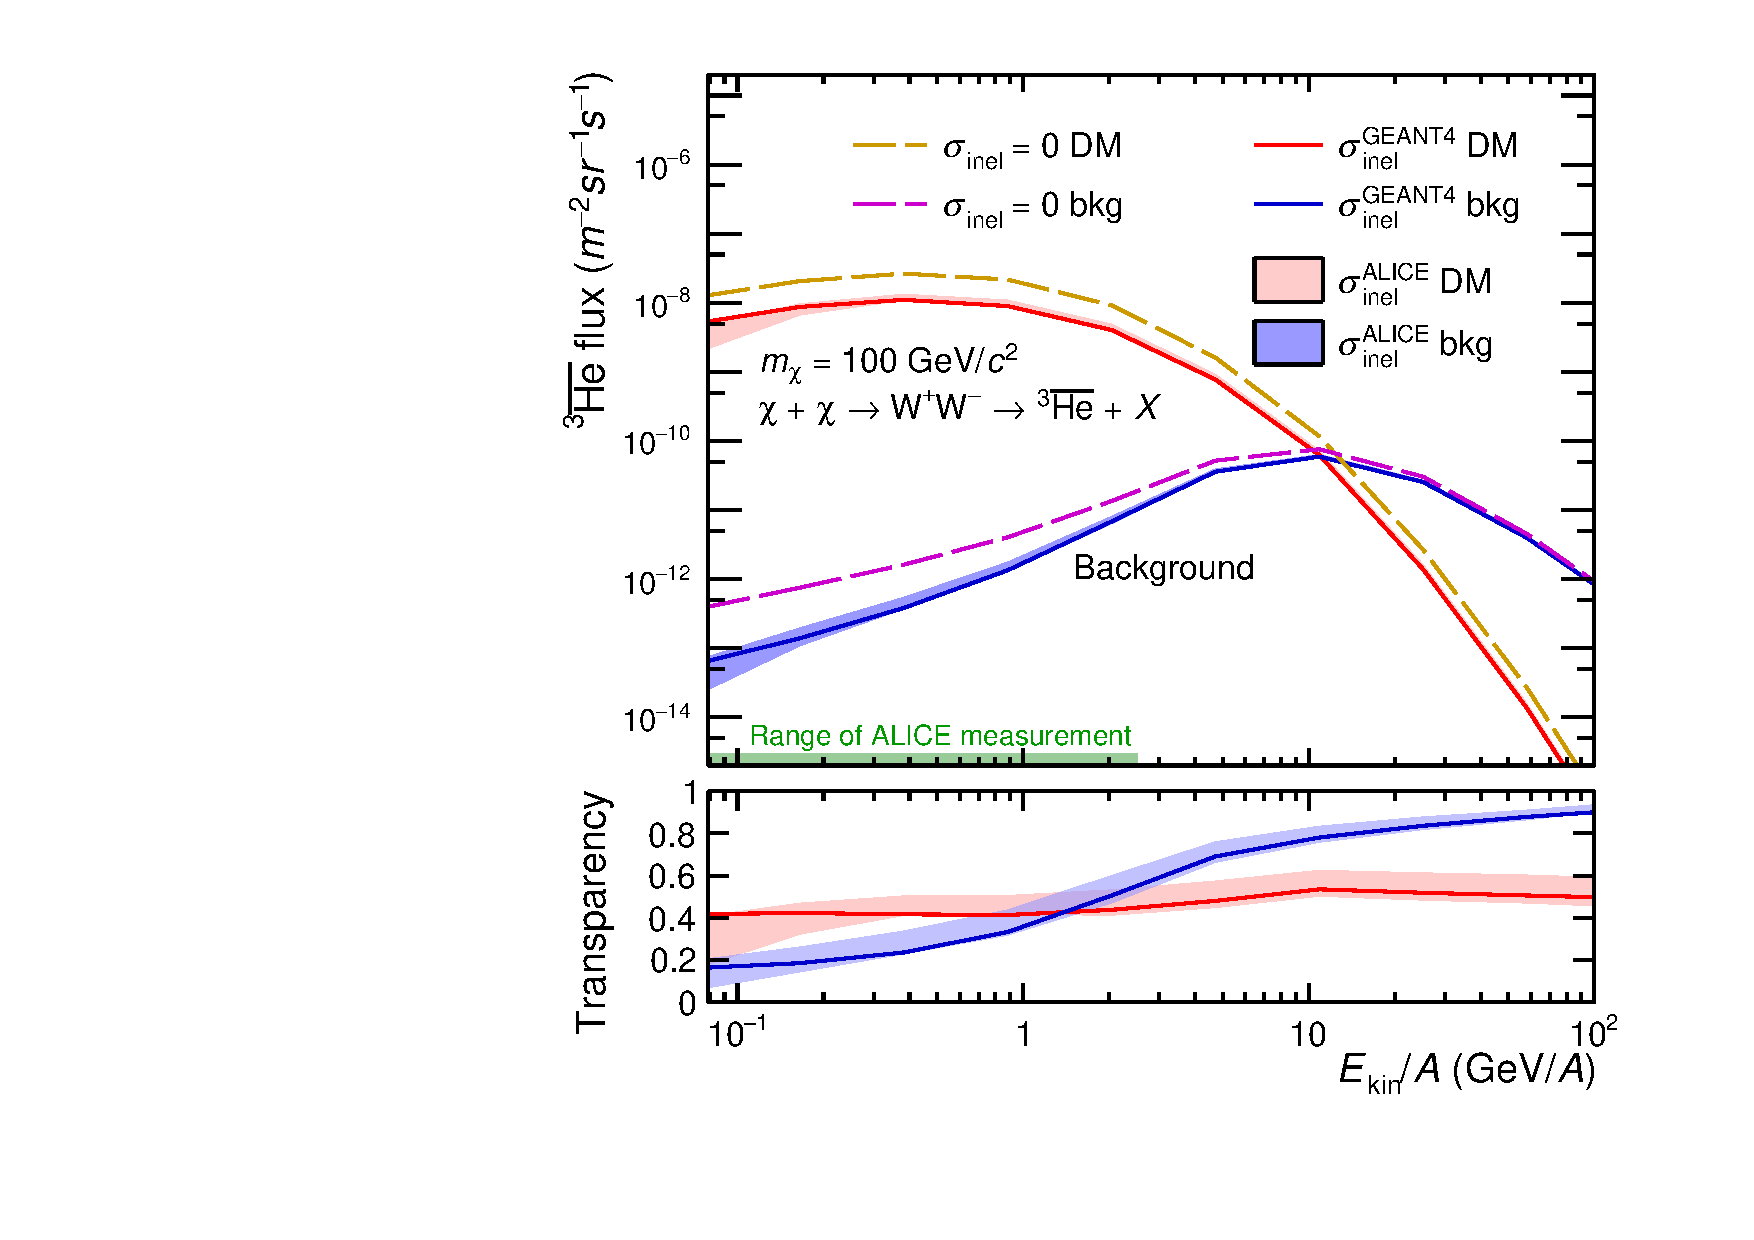
\includegraphics[width=0.45\textwidth]{figures/Antihelium_fluxes_LISWW_100GeV.pdf}
    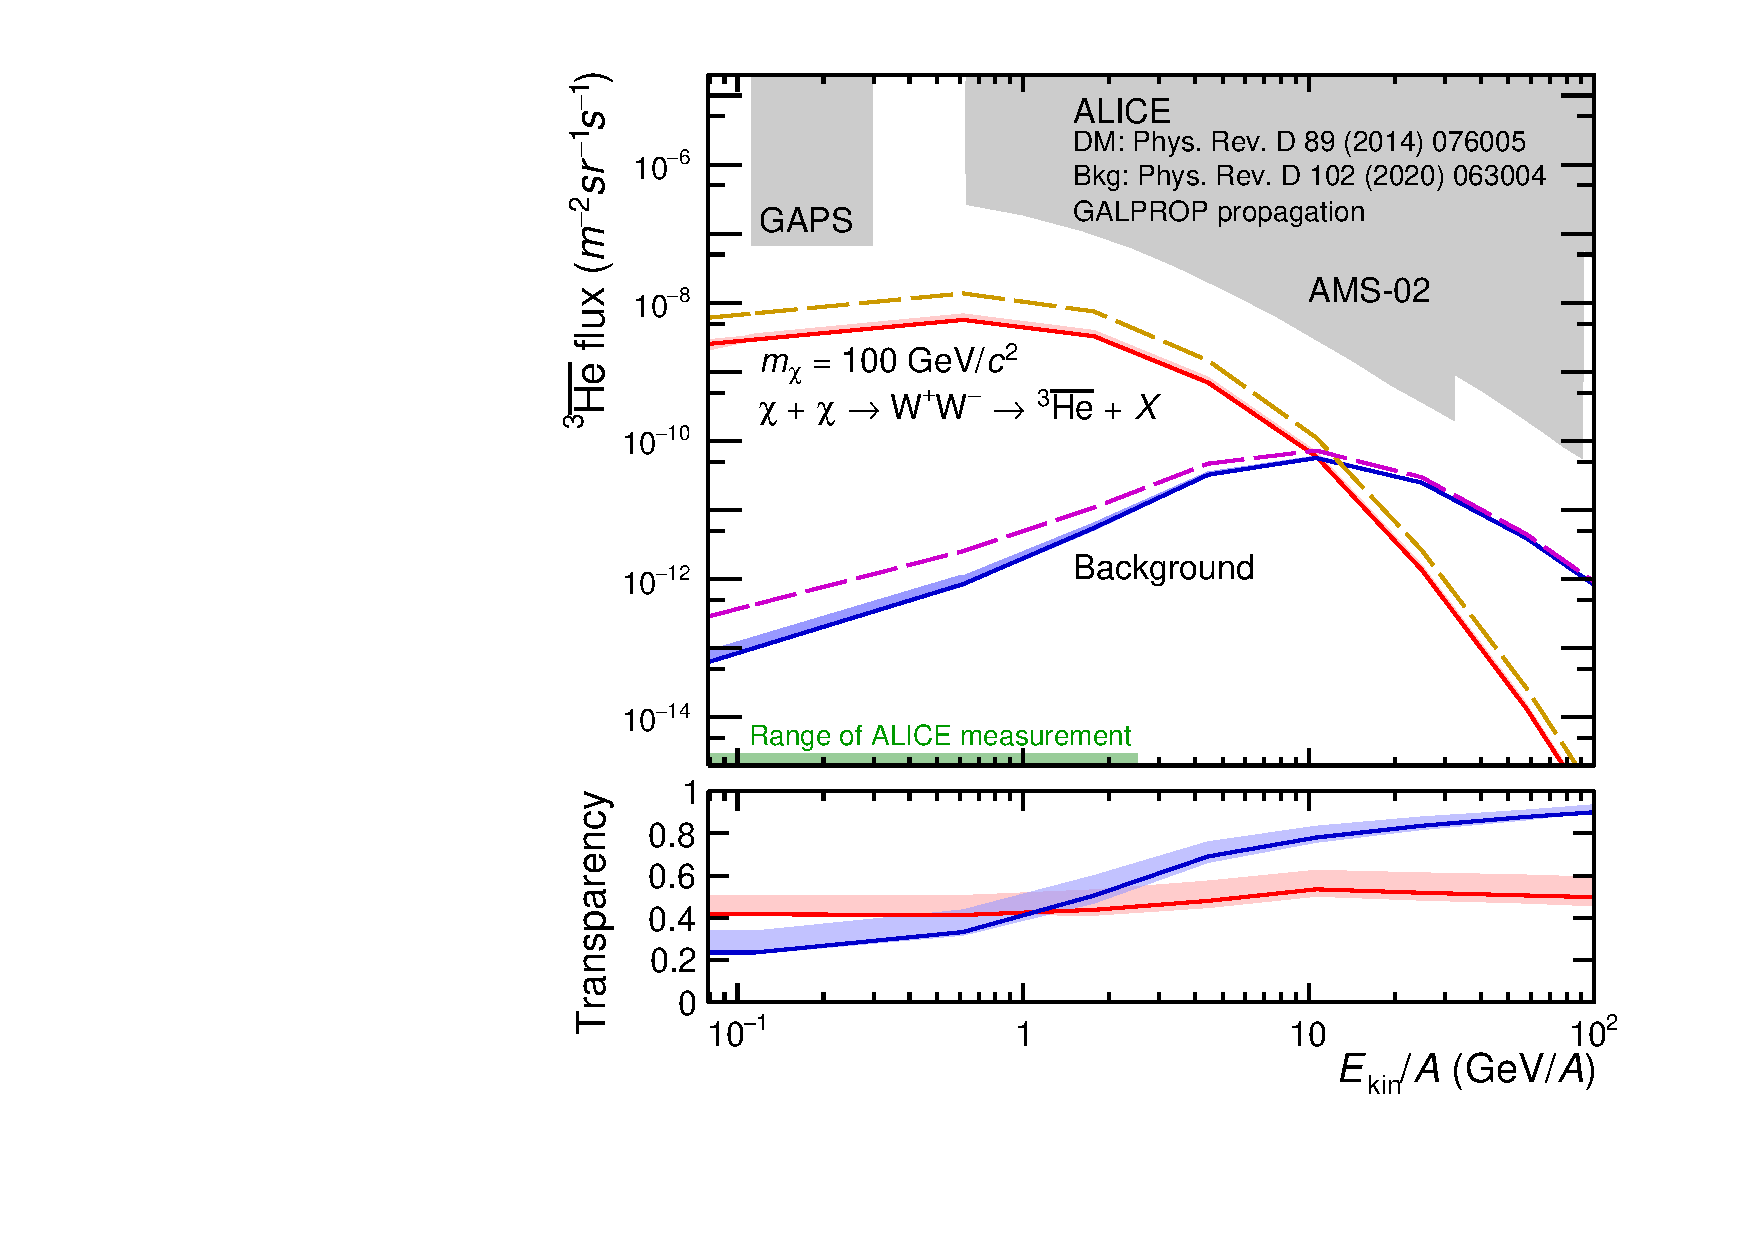
\includegraphics[width=0.45\textwidth]{figures/Antihelium_fluxes_solar_modulated_WW_100GeV.pdf}
    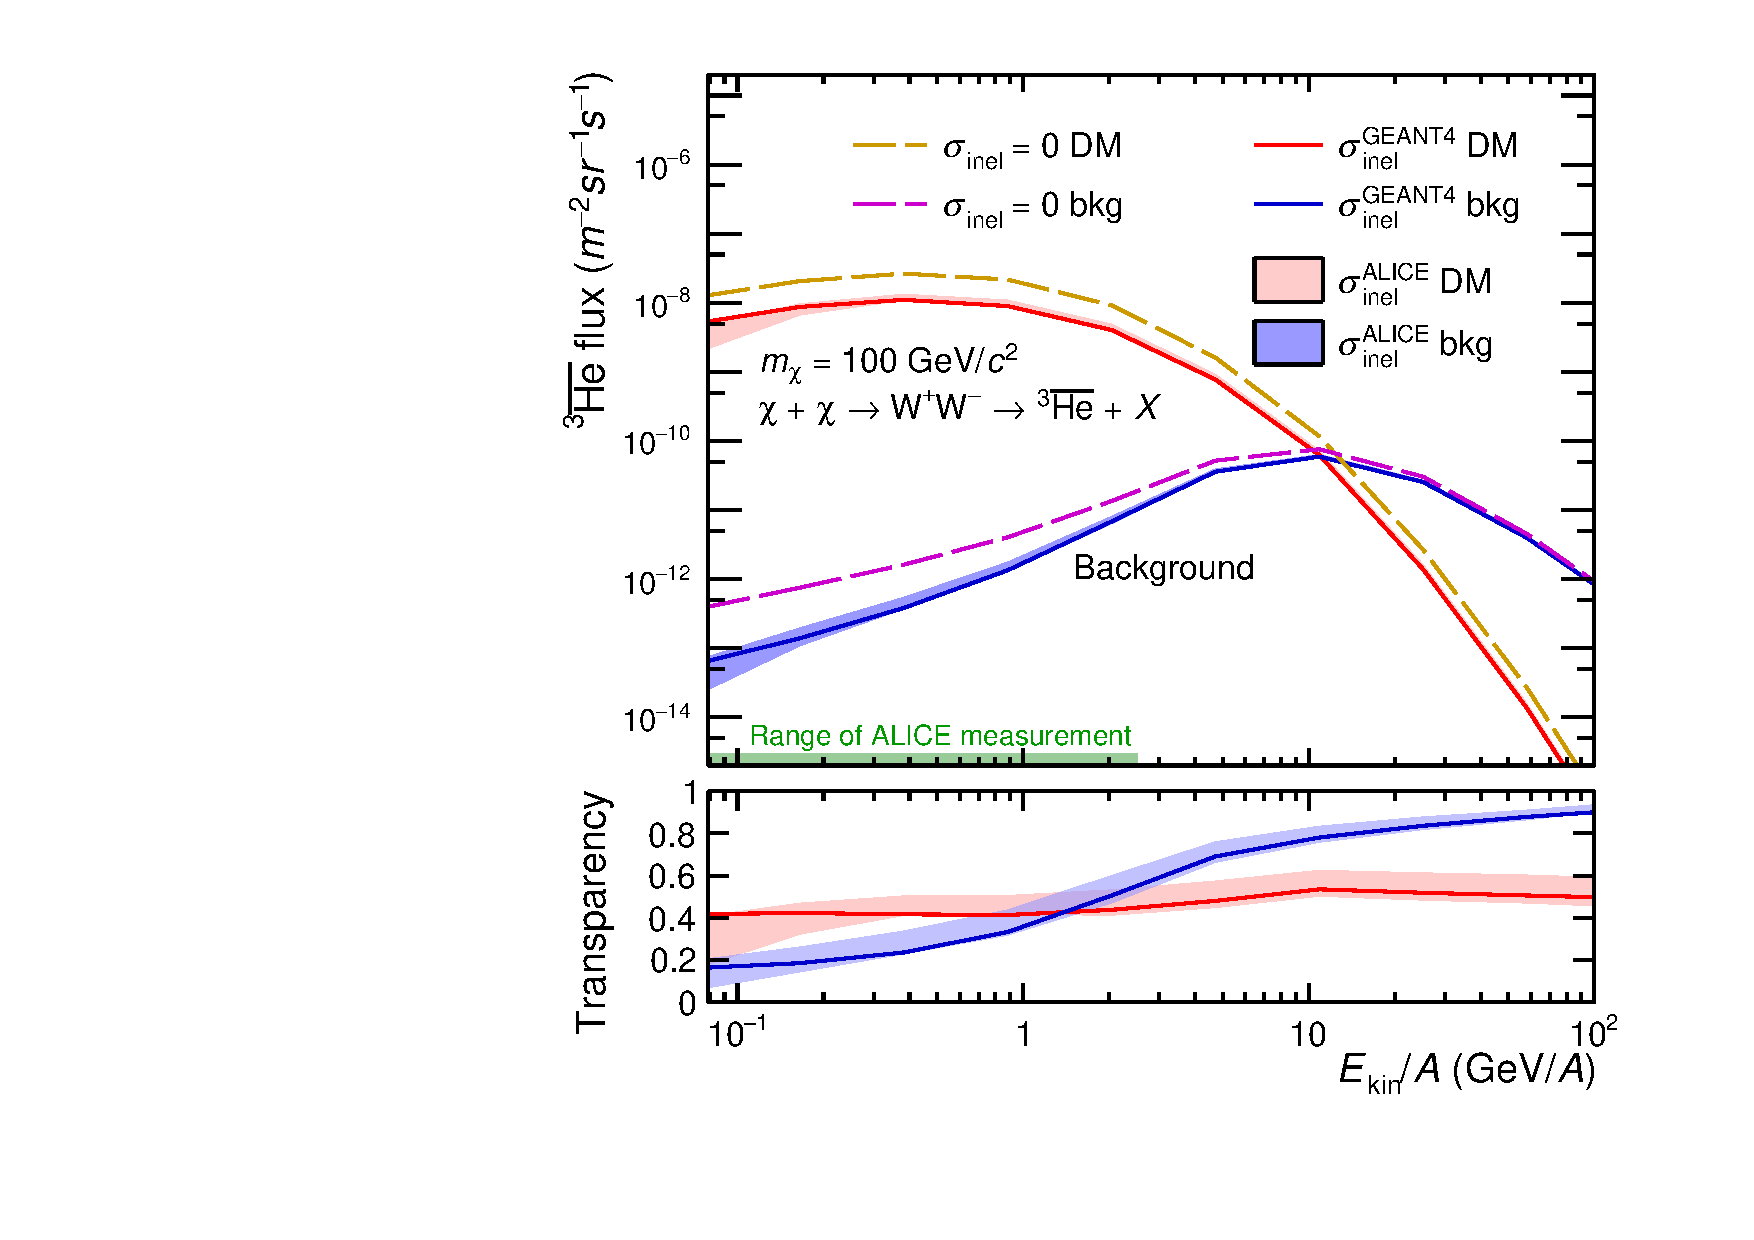
\includegraphics[width=0.45\textwidth]{figures/Antihelium_fluxes_LISWW_100GeV.pdf}
    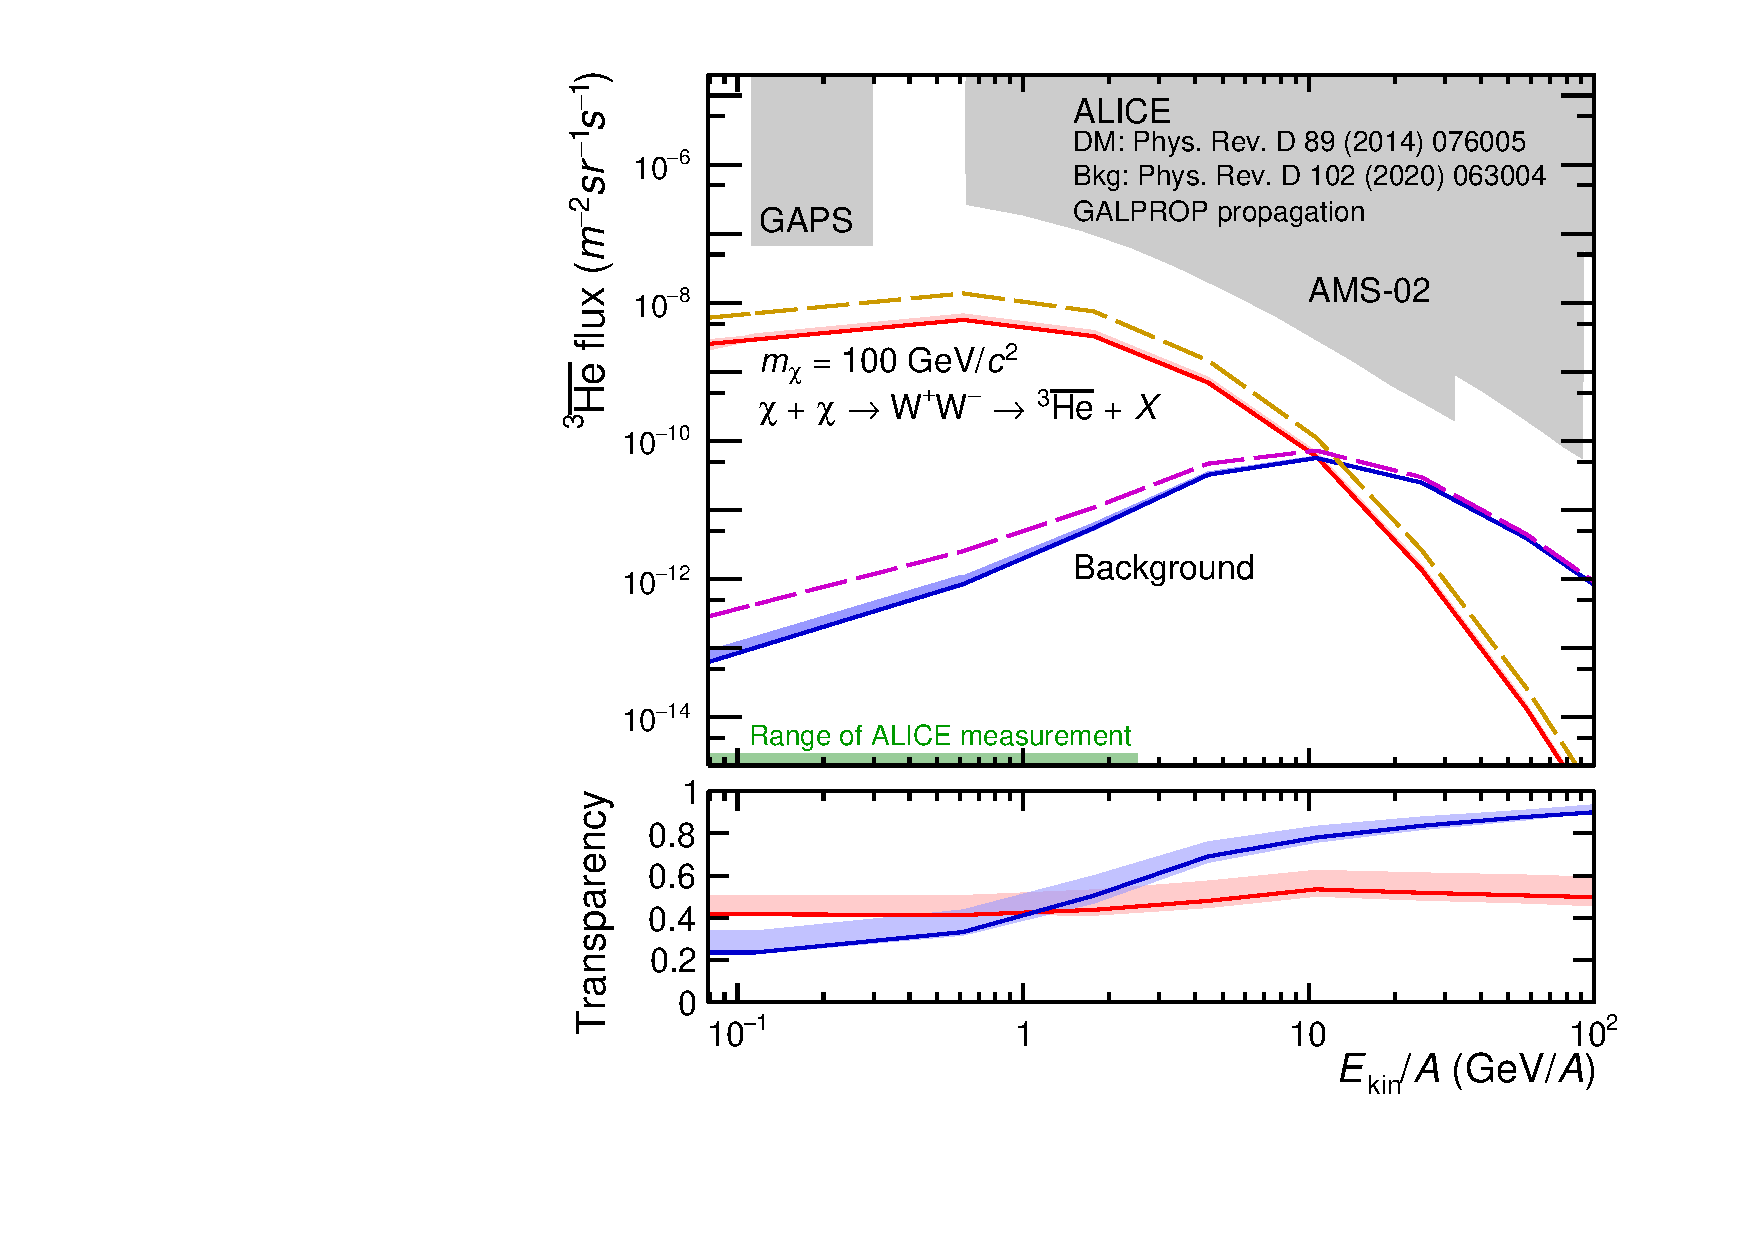
\includegraphics[width=0.45\textwidth]{figures/Antihelium_fluxes_solar_modulated_WW_100GeV.pdf}
    \caption{Expected \ahe\ fluxes for different \dmm\ ranging from 1GeV to 1TeV. They are compared to an expected spectrum of secondary \ahe\ from high energy cosmic ray collisions. The results are shown for the position of the solar system. The figures on the left show the results without solar modulation, and on the right with solar modulation included by means of a force field model, as is discussed in section \ref{sec:Propagation}. The results are also shown for different possible annihilation channels of dark matter, either through \WW\ (top) or through \bb\ (bottom).}
    \label{fig:Results_He3_fluxes_diff_DM_masses}
\end{figure}
\subsubsection{Results for different dark matter profiles}\label{sec:ResDMProfiles}
The effect of the different dark matter profiles is shown only on one channel and one dark matter mass, since it has similar effects on all channels/masses. The absolute normalization is degenerate with bounds from antiproton measurements, as was discussed in section \ref{sec:}. However, more insight can be gained from the bottom panel of figure \ref{fig:different_DM_profiles_and_transparencies}, the trasparency of the mikly way shows a significant shift between the three different profiles. This can be understood as the mean distance that antinuclei from dark matter have to traverse in order to get to earth. The more peaked the spectrum is towards the center, the longer the mean path. This in turn reduces the transparency. Thus, the transparency of the galaxy to antinuclei is lowest for the Einasto profile, which is the most peaked, as can be seen in figure \ref{fig:DM_profiles}. It is highest for the isothermal profile, which is relatively flat towards the centre of the mikly way. 

\begin{figure}
    \centering
    \includegraphics[width=0.8\textwidth]{}
    \caption{Caption}
    \label{fig:different_DM_profiles_and_transparencies}
\end{figure}


\subsection{Summary of propagation of antinuclei through the galaxy}
From the results in this section several conclusions can be drawn. The most impactful are the novel experimental uncertainties on the effect of the inelastic cross section on antinuclei propagation. These uncertainites are of the order of 1X\% for antihelium, and X\% for antideuterons, and thus significantly below the uncertainites from other effects, dominantly the uncertainty on the production of these antinuclei. The second conclusion is that the exact shape of the dark matter profile is a minor component in determining the normalization of antinuclei, even before possible degeneracies with antiproton limits are taken into account. This means that even though the dark matter profile is a free choice in current models, the final antinuclei fluxes are not sensitive to this.  The choice of the dark matter mass however has an important effect, both on the shape and the normalization of the resulting antinuclei spectrum. In particular for large WIMP masses, approching or exceeding masses of 1TeV, the shape of the spectrum becomes very similar to the shape of the secondary spectrum, which would make differentiation between them difficult. From the considered channels, only the $\Lambda_b$ boosted channel significantly deviated from the others, and only for \ahe\ , which however leaves open the possibility that other not thoroughly considered channels might influence the production of one antinucleus over another. If one were to speculate about the tentative antihelium events seen by the AMS collaboration, which are predominantly at high energies, they might originate from a heavy WIMP, with the \ahe\ production significantly boosted relative to antiproton and antideuteron productions, through some unknown mechanism. What is clear however, is that unraveling the mysteries of such a signal could do wonders for our understanding of antinuclei sources in our galaxy, and might even expose new physics.   



\subsection{Experiments to detect antinuclei in the cosmos}
Given their rarity, antinuclei in cosmic rays are difficult to detect. The experiment which currently has the best sensitivity for detecting antinuclei is AMS-02, which is a magnetic spectrometer on the international space station. As a magnetic spectrometer, AMS-02 is more sensitive to charge differences, and therefore more sensitive to \ahe\ nuclei than to antideuterons, since the latter need to be distinguished from the significalty more abundant antiprotons. However, it is still a big surprise that AMS has reported signals consistent with multiple \ahe\ nuclei, given that none of the currently available models predict a flux within the sensitivity of AMS, much less an order of magnitude above. These reports have cause a large amount of effort from both experimental and theoretical communities to come up with theories which might explain this signal, while also taking into account the lack of evidence for an antideuteron signal. It is currently unclear which process would produce such a large \ahe\ flux without boosting the antideuteron flux in a similar amount, with some suggested options being a boost to \ahe\ production via $\Lambda_b$ decays\cite{}. \\

There are also searched specifically designed to look for antideuterons
\subsubsection{Balloon and space bourne experiments}
Detecting antinuclei in cosmic rays has to be done near the top of our atmosphere, since antinuclei would annihilate well before reaching any ground based detector. This leaves either space bourne experiments or high altitude balloon flights. Currently there are two promising experiments either currently or soon to be deployed: the Alpha Magnetic Spectrometer (AMS) on the international space station (ISS), and the General AntiParticle Spectrometer (GAPS), which is a planned balloon flight experiment. The two are shortly discussed below.\\

The current generation of the AMS experiment -- AMS-02 -- has been analyzing cosmic rays since 2011, having analyzed over 200 billion cosmic ray events. It consists of several detector systems, including a Time-of-Flight detector, a silicon tracker, a star tracker (to determine its orientation), a transition radiation detector, a permanent magnet to curve charged particle tracks, a Cherenkov detector and an electromagnetic calorimeter. This makes its makeup similar to accelerator based detectors, such as ALICE. AMS has delivered incredibly precise data on cosmic ray spectra of nuclei up to heavy elements, as well for electrons, positrons and antiprotons. In particular the antiproton spectra have been studies extensively for hints of WIMP dark matter decays, as was already discussed in section \ref{sec:WIMPS}. \\
The "smoking gun" signal which AMS could detect from exotic physics such as dark matter would of course be an antinuclei signal. However, as could be seen from the plots in figure \ref{fig:Results_He3_fluxes_diff_DM_masses}, neither the expected flux from secondaries nor from the current WIMP dark matter models are expected to be able to reach the sensitivity of AMS. Therefore it is all the more interesting that AMS has repeatedly claimed the observation of multiple high energy \ahe\ and $^4\mathrm{\overline{He}}$ events \cite{}, but as of now these findings have not been published. These events have kinetic energies per nucleon above 10GeV/c. Should the claimed findings indeed be accurate, it comes with a few puzzling questions. Why is the flux so much greater than expected? This increase is unlikely to be the result of high energy cosmic ray collisions, as those are fairly well understood. They are however also significantly above the expected flux of most dark matter models. One study has concluded that the only standard model process that could plausibly produce such a flux would be an anti-star within 1kpc of earth\cite{}. This would however be very visible from gamma ray observations, as the large amounts of antimatter-matter annihilations would produce a distinct signal in the gamma ray spectrum\cite{}. As such, a confirmation of the reported signals would suggest a source beyond the standard model. One possible explanation would be dark matter, where the production of antinuclei is boosted by channels not yet considered. One such example is the recent study on antinuclei production through the $\overline{\Lambda_b}$ channel \cite{}. The second question these findings raise is the scaling of the antinuclei production with each additional nucleon. The number of \ahe\ to $^4\mathrm{\overline{He}}$ events observed suggest a ratio close to 1:3, whereas for production in small systems at the LHC the penalty factor is 1:1000. The final question -- and perhaps the easiest to answer -- is why 10s of \ahe\ events have been observed while AMS has yet to report a single antideuteron event. The most likely explaination for this question is simply that differentiating antideuterons from antiprotons is very difficult, as they have the same charge. The background from the antiproton signal might therefore simply cover the sensitivity to an antideuteron flux.\\

The current generation of the AMS experiment will hopefully continue to deliver data for years to come, however, planning for the next generation is already ongoing. This next generation experiment is called AMS-100, due to its planned acceptance of 100m$^2$sr. It will be a satellite experiment located at Lagrange point 2, using many of the same technologies and systems as the James-Webb-Space-Telescope (JWST). AMS-100 would have a 1000 fold increase in acceptance compared to AMS-02, and be able to deal with rigidities up to 100TV (AMS-02 up to 2TV). It will also employ a greater magnetic field, using high temperature superconductors \cite{}. As such, it is expected to deliver more precise measurements of antinuclei in cosmic rays, and thus shine light of the questions posed by current measurements.\\

GAPS is a more specialised detector, focused less on measuring all kinds of cosmic rays but rather specializing on detecting annihilation events of antimatter. To this end, a novel techinique is used to detect annihilations, called the "exotic atom" technique. The antiparticle travelling through the detector will loose energy due to Boethe-Bloch ionization until it stops, at which point it will displace an electron in an atom to form an exotic atom with near unit probability. The radiative decay of such an exited atom can be uniquely matched to the components of the exotic atom \cite{}. The benefit of antinuclei detection via balloon bourne experiments over sattelite bourne ones is the much reduced costs.\\

The main goal of GAPS is to measure any low-energy antideuteron flux, or improve on the current upper limit, and to follow up on the antihelium events reported by the AMS Collaboration. GAPS reach extends to lower energies than those probed by AMS, making such searches complementary. The expected sensitivity to antideuterons of GAPS of shown in figure \ref{fig:GAPS_sensitivity}, compared with AMS upper limits. As can be seen, the sensitivities are comparable. GAPS is also acting as a pathfinder for future balloon experiments by demonstrating such new technologies, and their usefulness for specific searches. 

\begin{figure}
    \centering
    \includegraphics{}
    \caption{Caption}
    \label{fig:GAPS_sensitivity}
\end{figure}




%\subsubsection{Developing a cubesat for detecting antiprotons}

